%%%%%%%%%%%%%%%%%%%%%%%%%%%%%%%%%%%%%%%%%%%%%%%%%%%%
%%%                                              %%%
%%%     Language Science Press Master File       %%%
%%%         follow the instructions below        %%%
%%%                                              %%%
%%%%%%%%%%%%%%%%%%%%%%%%%%%%%%%%%%%%%%%%%%%%%%%%%%%%
 
% Everything following a % is ignored
% Some lines start with %. Remove the % to include them

\documentclass[output=short% short|inprep              
%  	        ,draftmode  
%			,uscover
		  ]{langsci/langscibook}    
  
%%%%%%%%%%%%%%%%%%%%%%%%%%%%%%%%%%%%%%%%%%%%%%%%%%%%
%%%                                              %%%
%%%          additional packages                 %%%
%%%                                              %%%
%%%%%%%%%%%%%%%%%%%%%%%%%%%%%%%%%%%%%%%%%%%%%%%%%%%%

% put all additional commands you need in the 
% following files. {I}f you do not know what this might 
% mean, you can safely ignore this section

%%%%%%%%%%%%%%%%%%%%%%%%%%%%%%%%%%%%%%%%%%%%%%%%%%%%
%%%                                              %%%
%%%                 Metadata                     %%%
%%%          fill in as appropriate              %%%
%%%                                              %%%
%%%%%%%%%%%%%%%%%%%%%%%%%%%%%%%%%%%%%%%%%%%%%%%%%%%%

\title{New directions in corpus-based translation studies}  %look no further, you can change those things right here.
\subtitle{}
\BackTitle{New directions in corpus-based translation studies} % Change if BackTitle != Title
\BackBody{Corpus-based translation studies has become a major paradigm and research methodology and has investigated a wide variety of topics in the last two decades. The contributions to this volume add to the range of corpus-based studies by providing examples of some less explored applications of corpus analysis methods to translation research. They show that the area keeps evolving as it constantly opens up to different frameworks and approaches, from appraisal theory to process-oriented analysis, and encompasses multiple translation settings, including (indirect) literary translation, machine(-assisted) translation and the practical work of professional legal translators. The studies included in the volume also expand the range of application of corpus applications in terms of the tools used to accomplish the research tasks outlined.}
%\dedication{Change dedication in localmetadata.tex}
\typesetter{Claudio Fantinuoli, Katrin Hamberger, Felix Kopecky, Sebastian Nordhoff}
\proofreader{Željko Agić, Benedikt Baur, Rachele De Felice, Stefan Hartmann, Rebekah Ingram, Ka Shing Ko, Kristina Pelikan, Christian Pietsch, Daniela Schröder, Charlotte van Tongeren}
\author{Claudio Fantinuoli and Federico Zanettin}
\renewcommand{\lsSpineAuthor}{Fantinuoli \& Zanettin (eds.)}
\renewcommand{\lsISBNdigital}{978-3-944675-83-1}   % ISBN for the digital edition
\renewcommand{\lsISBNhardcover}{978-3-944675-74-9} % ISBN for the hardcover pritn
\renewcommand{\lsISBNsoftcover}{978-3-944675-75-6} % ISBN for the softcover print
\renewcommand{\lsISBNsoftcoverus}{978-1-523743-55-1} % ISBN for the softcover print
\renewcommand{\lsSeries}{tmnlp} % use lowercase acronym, e.g. sidl, eotms, tgdi
\renewcommand{\lsSeriesNumber}{1} %will be assigned when the book enters the proofreading stage
\renewcommand{\lsURL}{http://langsci-press.org/catalog/book/76} % contact the coordinator for the right number

%\renewcommand{\lsCoverTitleFont}[1]{\sffamily\addfontfeatures{Scale=MatchUppercase}\fontsize{49pt}{16.75mm}\selectfont #1} 
% add all extra packages you need to load to this file  
\usepackage{tabularx} 

%%%%%%%%%%%%%%%%%%%%%%%%%%%%%%%%%%%%%%%%%%%%%%%%%%%%
%%%                                              %%%
%%%           Examples                           %%%
%%%                                              %%%
%%%%%%%%%%%%%%%%%%%%%%%%%%%%%%%%%%%%%%%%%%%%%%%%%%%% 
%% to add additional information to the right of examples, uncomment the following line
% \usepackage{jambox}
%% if you want the source line of examples to be in italics, uncomment the following line
% \renewcommand{\exfont}{\itshape}
\usepackage{./langsci/styles/langsci-gb4e}
\usepackage{listings}

\lstset{ %
  backgroundcolor=\color{white},   % choose the background color; you must add \usepackage{color} or \usepackage{xcolor}
  basicstyle=\footnotesize\ttfamily,        % the size of the fonts that are used for the code 
  keywordstyle=\color{blue!60!black},       % keyword style
  language=XML,                 % the language of the code 
  stringstyle=\color{green!60!black},     % string literal style 
  morekeywords={token,xlink:href, Action, Value, Cursor,LogEvent}
} 

% \usepackage[final]{pdfpages}
 

%% hyphenation points for line breaks
%% Normally, automatic hyphenation in LaTeX is very good
%% If a word is mis-hyphenated, add it to this file
%%
%% add information to TeX file before \begin{document} with:
%% %% hyphenation points for line breaks
%% Normally, automatic hyphenation in LaTeX is very good
%% If a word is mis-hyphenated, add it to this file
%%
%% add information to TeX file before \begin{document} with:
%% %% hyphenation points for line breaks
%% Normally, automatic hyphenation in LaTeX is very good
%% If a word is mis-hyphenated, add it to this file
%%
%% add information to TeX file before \begin{document} with:
%% \include{localhyphenation}
\hyphenation{
affri-ca-te
affri-ca-tes
com-ple-ments
}
\hyphenation{
affri-ca-te
affri-ca-tes
com-ple-ments
}
\hyphenation{
affri-ca-te
affri-ca-tes
com-ple-ments
}
%\bibliography{localbibliography} 

%%%%%%%%%%%%%%%%%%%%%%%%%%%%%%%%%%%%%%%%%%%%%%%%%%%%
%%%                                              %%%
%%%             Frontmatter                      %%%
%%%                                              %%%
%%%%%%%%%%%%%%%%%%%%%%%%%%%%%%%%%%%%%%%%%%%%%%%%%%%% 
\begin{document}     
\year=2015
%add all your local new commands to this file

\newcommand{\smiley}{:)}

\renewbibmacro*{index:name}[5]{%
  \usebibmacro{index:entry}{#1}
    {\iffieldundef{usera}{}{\thefield{usera}\actualoperator}\mkbibindexname{#2}{#3}{#4}{#5}}}

% \newcommand{\noop}[1]{} 
 
\maketitle                
\frontmatter
% %% uncomment if you have preface and/or acknowledgements

%\currentpdfbookmark{Contents}{name} % adds a PDF bookmark
%\tableofcontents
% \addchap{Preface}
\begin{refsection}

%content goes here

\printbibliography[heading=subbibliography]
\end{refsection}

% \include{chapters/acknowledgments}
% \include{chapters/abbreviations} 
\mainmatter         
  

%%%%%%%%%%%%%%%%%%%%%%%%%%%%%%%%%%%%%%%%%%%%%%%%%%%%
%%%                                              %%%
%%%             Chapters                         %%%
%%%                                              %%%
%%%%%%%%%%%%%%%%%%%%%%%%%%%%%%%%%%%%%%%%%%%%%%%%%%%%
 
%\documentclass[output=paper]{LSP/langsci}
\author{Tatiana Serbina, Paula Niemietz and Stella Neumann}
\title{Development of a keystroke logged translation corpus}
%\epigram{Change epigram in chapters/01.tex or remove it there }
\abstract{This paper describes the development of a keystroke logged translation corpus containing both translation product and process data. The initial data comes from a translation experiment and contains original texts and translations, plus the intermediate versions of the unfolding translation process. The aim is to annotate both process and product data to be able to query for various features and recurring patterns. However, the data must first be pre-processed to represent individual keystroke logging events as linguistic structures, and align source, target and process units. All process data, even material that does not appear in the final translation product, is preserved, under the assumption that all intermediate steps are meaningful to our understanding of the translation process. Several examples of possible data queries are discussed to show how linguistically informed quantitative analyses of the translation process data can be performed.}
\maketitle

\begin{document}
 
\section{Introduction} \label{sec:1:1}
Empirical translation studies can be subdivided into two main branches, namely product and process-based investigations \citep[see][]{Laviosa2002,Göpferich2008}. Traditionally, the former are associated with corpus studies, while the latter require translation experiments. The present study combines these two perspectives on translation by treating the translation process data as a corpus and tracing how linguistic phenomena found in the final product have developed during the translation process.

Typically, product-based studies consider translations as texts in their own right, which can be analyzed in terms of translation properties, i.e. ways in which translated texts systematically differ from the originals. The main translation properties analyzed so far include simplification, explicitation, normalization towards the target text (\textsc{tt}), leveling out \citep{Baker1996} and shining through of the source text (\textsc{st}) \citep{Teich2003}. Investigations into these properties can be conducted using monolingual comparable corpora containing originals and translations within the same language \citep[e.g.][]{Laviosa2002}, bilingual parallel corpora consisting of originals and their aligned translations \citep[e.g.][]{Becher2010}, or also combinations of both \citep{Culo2012,Hansen-Schirra2012}.

Empirical research requires not only description but also explanation of translation phenomena. Why, for instance, are translated texts more explicit than originals? It has been suggested that explicitation as a feature of translated texts is a rather heterogeneous phenomenon and can be subdivided into four different types: the first three classes are linked to contrastive and cultural differences, whereas instances of the fourth type are specific to the translation process \citep[82--83]{Klaudy1998}. Other researchers propose to explain translation phenomena in general through contrastive differences between \textsc{st} and \textsc{tt}, register characteristics and a set of factors connected to the translation process, for instance those related to the process of understanding \citep{Steiner2001}. Thus, studies using parallel corpora have shown that the majority of examples of explicitation found in the data can be accounted for through contrastive, register and/or cultural differences \citep{Hansen-Schirra2007,Becher2010}. Based on these corpus-based studies researchers can formulate hypotheses that ascribe the remaining instances to the characteristics of the translation process, and then test these hypotheses by considering data gathered during translation experiments, e.g. through keystroke logging. Keystroke logging software such as \textit{Translog} \citep{Jakobsen1999} allows researchers to study intermediate steps of translations by recording all keystrokes and mouse clicks during the process of translation. Based on this behavioral data and the intermediate versions of translations, assumptions with regard to cognitive processing during translation can be made. Analysis of translation process data helps explain the properties of translation products, describe potential translation problems and identify translation strategies.

Previous studies in this area have focused on analysis of pauses and the number as well as length of the segments in between \citep[e.g.][]{Dragsted2005,Jakobsen2005,Alves2009,Alves2011}. Furthermore, translation styles have been \enlargethispage{1\baselineskip} investigated in both quantitative and qualitative manners \citep[e.g.][]{Pagano2008, CarlandDragsted2011}, for example, the performances of professional and student translators have been compared with regard to speed of text production during translation, length of produced chunks and revision patterns \citep[e.g.][]{Jakobsen2005}.
 
In order to generalize beyond individual translation sessions and individual experiments, keystroke logging data has to be treated as a corpus \citep{Alves2004, Alves2009, Alves2011}. In other words, the data has to be organized in such a way as to allow querying for specific recurring patterns \citep{Carl2009} which can be analyzed both in terms of extra-linguistic factors such as age and gender of the translator, or time pressure, as well as linguistic features such as level of grammatical complexity, or word order. The latter research questions require additional linguistic annotation of the keystroke logging data (see \sectref{sec:1:2:3}). Thus, the aim of the present study is to create a keystroke logged corpus (\textsc{klc}) and to perform linguistically informed quantitative analyses of the translation process data.

\sectref{sec:1:2} describes the translation experiment data which serves as a prototype of a keystroke logged corpus, as well as the required pre-processing and linguistic annotation necessary for corpus queries, which are introduced in \sectref{sec:1:3}. A summary and a short outlook are provided in \sectref{sec:1:4}.\footnote{The project e-cosmos is funded by the Excellence Initiative of the German State and Federal Governments.} 

\section{Keystroke logged translation corpus} \label{sec:1:2}
\subsection{Data} \label{sec:1:2:1}

The first prototype of the keystroke logged translation corpus is based on the translation process data collected in the framework of the project \textsc{probral}\footnote{The project was funded by \textsc{capes}--\textsc{daad} \textsc{probral} (292/2008).} in cooperation with the University of Saarland, Germany and the Federal University of Minas Gerais, Brazil. In the translation experiment participants were asked to translate a text from English into German (their L1). No time restrictions were imposed. The data from 16 participants is available: eight of them are professional translators with at least two years of experience and the other eight participants are PhD students of physics. Since the source text is an abridged version of an authentic text dealing with physics (see Appendix), the second group of participants are considered domain specialists. The original text was published in the popular-scientific magazine \textit{Scientific American Online}, and the translation brief involved instructions to write a translation for another popular-scientific publication. The text was locally manipulated by integrating ten stimuli representing two different degrees of grammatical complexity, illustrated in \REF{ex:1:1} and \REF{ex:1:2}. Based on previous research in Systemic Functional Linguistics (see \citealt[715]{Halliday2014}; \citealt[8--10]{Taverniers2003}), we assume that in the complex version the information is more dense and less explicit. For instance, whereas the italicized stretches of text in \REF{ex:1:1} and \REF{ex:1:2} contain the same semantic content, its realization as a clause in \REF{ex:1:1} leads to an explicit mention of the agents, namely the researchers, which are left out in the nominalized version presented in \REF{ex:1:2}. During the experiment every participant translated one of the two versions of the text, in which simple and complex stimuli had been counterbalanced. In other words, five simple and five complex stimuli integrated into the first source text corresponded to the complex and simple variants of the same stimuli in the second text. The only translation resource allowed during the translation task was the online bilingual dictionary \textit{leo}.\footnote{\url{http://dict.leo.org/ende/index_de.html}.} The participants’ keystrokes, mouse movements and pauses in between were recorded using the software \textit{Translog}. Additionally, the information on gaze points and pupil diameter was collected with the help of the remote eye-tracker \textit{Tobii 2150}, using the corresponding software \textit{Tobii Studio}, version 1.5 \citep{Tobii2008}. Currently the corpus considers only the keystroke logging data, but later the various data sources will be triangulated \citep[see][]{Alves2003} to complement each other. The discussion of individual queries and specific examples in \sectref{sec:1:3} indicates how the analysis of the data could benefit from the additional data stream. 

\ea \label{ex:1:1} Simple stimulus\\
Instead of collapsing to a final fixed size, the height of the crushed ball continued to decrease, even three weeks \emph{after the researchers had applied the weight}. (\textsc{Probral} Source text 2)
\z

\ea \label{ex:1:2}
Complex stimulus\\
Instead of collapsing to a final fixed size, the height of the crushed ball continued to decrease, even three weeks \emph{after the application of weight}. (\textsc{Probral} Source text 1)
\z

The prototype of the \textsc{klc} thus consists of 2 versions of the original (source texts), 16 translations (target texts) as well as 16 log files (process texts). The source and target texts together amount to approximately 3,650 words, not including the process texts. The total size, taking into account various versions of the same target text words, can be determined only after completion of the pre-processing step (see \sectref{sec:1:2:2}). All the texts belong to the register of popular scientific writing. After the gold standard is established, the corpus will be extended to include data from further translation experiments, e.g. data stored in the \textsc{critt} \textsc{tpr--db} \citep{Carl2012}.\footnote{The \textsc{critt} \textsc{tpr--db} is the Translation Process Research Database of the Centre for Research and Innovation in Translation and Translation Technology.} This database is a collection of keystroke logging and eye-tracking data recorded during translation, editing and post-editing experiments. It provides both raw and processed data: for instance, originals and final translation products are tokenized, aligned and annotated with parts of speech, whereas the process data is analyzed in terms of gaze and keystroke units \citep{Carl2012}. According to the website, the current version of the database consists of approximately 1300 experiments.\footnote{\url{https://sites.google.com/site/centretranslationinnovation} .} In the development of our keystroke logged translation corpus we go further by identifying all potential tokens produced during a translation process and enriching these with linguistic information. At the moment, the relatively small size of the corpus is sufficient to develop the new procedures and queries required for this type of data. 

\subsection{Pre-processing} \label{sec:1:2:2}
While the originals and the final translations can be automatically annotated and aligned using existing tools, the process texts require pre-processing before they can be enriched with further information. The keystroke logs consist of individual events corresponding to one press of a key or a mouse. To link this behavioral information to the linguistic level of analysis, the events have to be represented in terms of complete tokens. Since the intentions of a translator are not always clear, it is essential to reflect all possible tokens produced during the translation process. Using a modified version of the concept of target hypotheses that \citet{Lüdeling2008} introduced for learner corpora (which also contain non-standard language with errors), the \textsc{klc} will include multiple layers of annotation reflecting different versions of the same tokens that could be inferred from the process data. Thus, in our context, target hypotheses represent potential translation plans. Several hypotheses are annotated when the keystroke logging data is ambiguous, i.e. in cases when, based on the pressed keys, it is unclear what token the translator intended to produce, and when the process contains additional indicators of increased cognitive processing such as longer pauses or corrections. This method retains the necessary level of objectivity because it does not force the researcher to select only the version which appears most plausible at a certain stage of corpus compilation.

\citet{Leijten2012} discuss the processing of monolingual keystroke logging data by aggregating it from the character (keystroke) to the word level \citep[see also][]{Macken2012}. For translation data, however, the required processing is more complex. Within the target text keystrokes are aligned to tokens, and these tokens (representing intermediate versions of words either preserved in the \textsc{tt}, or modified/deleted in the process) are in turn aligned to the alignment units consisting of \textsc{st}--\textsc{tt} counterparts \citep[see][227]{Carl2009a}. The same process of alignment is also performed for the phrase and grammatical function levels. These alignment links make it possible to query for all intermediate versions of individual tokens and phrases (see \sectref{sec:1:3:5}).

To facilitate this alignment, an alignment tool was developed which allows the researcher to manually select items to be aligned from the \textsc{st} and the \textsc{tt}.\footnote{The tool was developed by students Adjan Hansen-Ampah (\textsc{rwth} Aachen) and Chuan Yao (Georgia Institute of Technology) during a \textsc{urop} project at \textsc{rwth} Aachen University in 2013.} These alignment units are saved in the same keystroke logging file. The screenshot in \figref{fig:1:1} shows the selection of an alignment pair with the tool: the words \textit{explaining }from the \textsc{st} list and \textit{erklären} `to explain' from the \textsc{tt} list are highlighted to become alignment pair 0 in the bottom window. The window on the left part of the screen displays the \textsc{xml} file for reference.


\begin{figure}
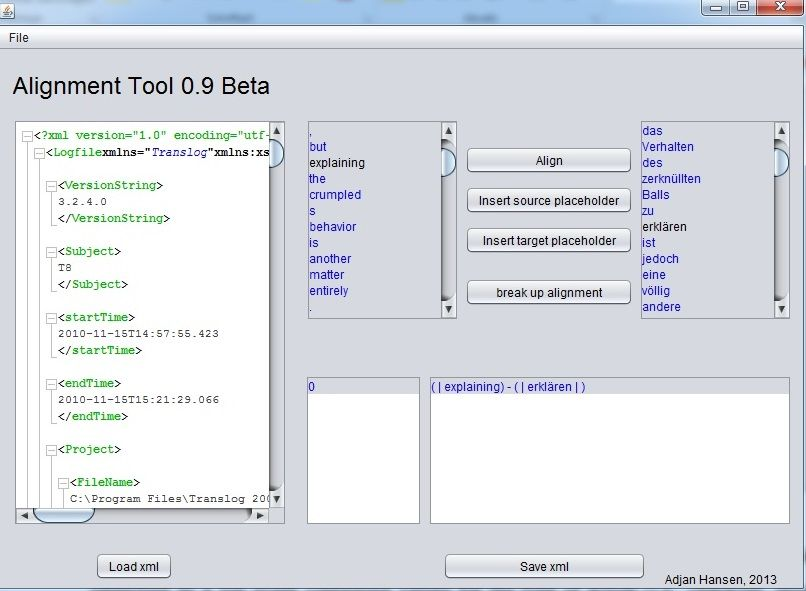
\includegraphics[width=.7\textwidth]{./figures/2-1.jpg}
\caption{Screenshot of an alignment process using the alignment tool} \label{fig:1:1}
\end{figure}


The \textit{Translog} software supplies the keystroke data in \textsc{xml} format. Each keystroke is identified as a log event containing values for the type of action (i.e., character, deletion, movement, mouse click), the cursor position of this keystroke, a time stamp and a block ID which identifies the number of characters highlighted in the log event (e.g. when a segment is highlighted prior to being moved or deleted). During the pre-processing stage for the prototype, the \textsc{xml} data was enriched by aggregating the log events into plausible tokens to which token IDs were assigned. For each alignment level (currently only word level; in the future also phrase and grammatical function levels) a reference link was specified to link the object to the corresponding alignment unit created by the aligner. If the token did not appear in the final version and could not be linked to any existing alignment units, the reference link was designated as an empty link. In example \REF{ex:1:3} below the three words \textit{für Verwirrung sorgt} `causes confusion', which appear in an intermediate version of this sentence, are characterized by empty links: since the same semantic information is expressed in the final version through a different grammatical structure using non-related lexical items, namely \textit{nicht vollständig erklären können} `could not explain entirely', the tokens cannot be connected to any alignment units. The reference to the empty links ensures that the information contained in the intermediate versions is preserved in the data and can be queried. These tokens can only be linked on the level of units larger than words. The frequent use of semantically equivalent structures rather than structurally similar units requires alignment on multiple levels, as certain relations cannot be captured at the level of individual words.\footnote{The intermediate versions of German translations use special characters introduced in linear representation, a visualization option provided by the keystroke logging software \textit{Translog}. {\raute} -- a space character, {\stern} --  approx. 1 sec. pause, [{\stern}36.721] -- a pause of 36 seconds, 721 milliseconds,{\pfeil} -- a backspace character. The part of the original corresponding to the translation is written in italics. One or more intermediate versions (GT\_i) and the final version (GT\_f) of translations, if relevant for the discussion, are presented in their chronological order.}

\ea \label{ex:1:3}
\begin{xlist}
\exi{}[\textbf{EO:}~~]{\upshape Yet it displays surprising strength and resists further compression, \emph{a fact that has confounded physicists}. (\textsc{probral})}
\exi{}[\textbf{GT\_i:}]{
\gll \raute\stern\stern{} eine{\raute} Tatsache,{\raute} die{\raute} Physikerf\raute\stern\pfeil\pfeil\raute{\color{red}[{\stern}11.968]}\pfeil\pfeil\pfeil\pfeil\pfeil\pfeil\pfeil\pfeil\pfeil{} bei\raute{} Physikern\raute{} für\raute{} Verwirrung\raute{} sorgrt\pfeil\pfeil{}t.\\
 {} a fact the physicists~ by physicists for confusion caters\\
}
\exi{}[\textbf{GT\_f}]{
\gll  eine Tatsache, die sich Physiker noch immer nicht vollständig erklären können\\
  a fact that themselves physicists yet still not entirely explain can\\
}
\end{xlist}
\z
%\exewidth{GTIIII}

\newpage
Similarly, empty links were also defined in the \textsc{st}--\textsc{tt} alignment units, if no corresponding element could be identified for either the \textsc{st} or the \textsc{tt} \citep{Culo2012}, so that this information can also be extracted from the corpus.    

\subsection{Annotation} \label{sec:1:2:3}
“Corpus annotation adds value to a corpus in that it considerably extends the range of research questions that a corpus can readily address” \citep[29]{McEnery2006}: a systematic annotation of particular information types throughout a corpus enables researchers to search for and extract corpus examples based on certain criteria included in one or more annotation layers. At the moment all texts are annotated with meta-information specifying the participant ID, a version of the translated text and the participant's group (translator/physicist). The meta-information will be extended to include further variables relevant for potential analyses of the translation process data, e.g. participant-specific metadata such as age or native language \citep[see][]{Hvelplund2012}. Furthermore, the \textsc{klc} will contain several layers of linguistic annotation. The part of speech (\textsc{pos}) annotation of the process texts was done manually for some examples in the corpus prototype, but the aim is to perform this step automatically for process as well as source and target texts through the use of an existing tagger. Automatic syntactic parsing and annotation of grammatical functions is also planned;\footnote{Different taggers and parsers will be tested, and in a later step trained to accommodate the non-standard features present in the \textsc{klc}. The ongoing work on pre-processing and annotation of monolingual process data \citep{Leijten2012,Macken2012} is being taken into consideration.} however, it is recognized that manual interaction to check the results will still be necessary. The multilayer annotation \citep[see][]{Hansen-Schirra2006} will be extended by integrating the target hypotheses as a separate annotation layer (see \sectref{sec:1:3:2}). In addition, behavioral information such as the length of individual pauses \citep[see][]{Alves2009,Alves2011} will be annotated to facilitate quantifying these types of features, as well as querying for a combination of behavioral and linguistic information.

\section{Possible queries} \label{sec:1:3}
Depending on the research questions, different types of queries into the translation process data are required. The following sub-sections describe a selection of possible queries. Taking into account the novelty of this corpus type for translation process research, this section aims at showing the potential applications of the planned annotation and alignment layers introduced above for the analysis of translations.

\subsection{Alternative versions and incomplete structures within individual intermediate versions} \label{sec:1:3:1}
One query type concerns alternative versions of an unfolding target text. During the process of translation, evolving texts typically undergo multiple revisions (e.g. in the form of deletions, overwrites or additions) before the final product is completed. One way of looking at revisions is to consider all keystrokes related to the translation of one source text sentence, up to the point where the translator begins translating other sentences, as an intermediate version of the translation of this source text sentence. The next version is identified, when and if the translation of this sentence is resumed after text production and/or revision of other passages.\footnote{The identification of intermediate versions differs from the annotation of different target hypotheses (see \sectref{sec:1:3:2}): for instance, in \REF{ex:1:4}, one intermediate version corresponds to two target hypotheses.} Often such intermediate versions could function on their own: their linguistic structures are complete and could be left unchanged throughout the translation session. However, for various reasons, subsequent revisions may lead to (a series of) changes in these structures, thus creating new versions of the same sentences.

A single intermediate version may include several alternatives for the same linguistic slot realized by the same part of speech. For example, in \REF{ex:1:4}, two versions of the modal verb within a subordinate clause have been supplied by the translator: the first of these in the present (\textit{können} `can') and the second in the past tense (\textit{konnten} `could'), separated by a slash.


\judgewidth{GTI:}
\ea \label{ex:1:4}
\begin{xlist}
\exi{}[\textbf{EO:~~}]{\emph{Yet it displays surprising strength and resists} further compression, a fact that has confounded physicists. (\textsc{probral})}
\exi{}[\textbf{GT\_i:}]{
\gll  [{\dots}] die\raute{} sich\raute{} Physiker\raute{} nicht\raute{} erklären\raute{} können\stern{}/konnten.\\
{}  which themselves physicists not explain can/could\\
}
\end{xlist}
\z

The part of speech annotation allows us to query this and similar patterns through a search for identical parts of speech separated by a punctuation mark. 
\figref{fig:1:2} shows the \textsc{xml} code provided by the keystroke logging software \textit{Translog} corresponding to the production of the tokens \textit{können} and \textit{konnten} in example \REF{ex:1:4}. As can be seen, the tool generates files representing one log event (e.g. a keystroke corresponding to a letter or a slash) per line. The pre-processing step requires the grouping of these events into tokens, such as \textit{können} and \textit{konnten}, which can be then annotated with part of speech tags. Here we use the tags from the Stuttgart-Tübingen Tagset (\textsc{stts}) for German \citep{Schiller1999} for the purposes of illustration. Both \textit{können} `can' in Token 38 and \textit{konnten} `could' in Token 40 bear the part of speech tag \textsc{vmfin} indicating `verb finite, modal'. 


\begin{figure}[t]

\caption{\textsc{xml} code enriched with alignment links and information on tokens and parts of speech} \label{fig:1:2}
\begin{lstlisting}
<t id="38" token="können" xlink:href="tAlign#28" xlink:href="emptylink#5">
    <LogEvent Action="1" Value="107" Cursor="477" Block="0" Time="00:04:59:694" />
    <LogEvent Action="1" Value="246" Cursor="478" Block="0" Time="00:04:59:850" />
    <LogEvent Action="1" Value="110" Cursor="479" Block="0" Time="00:05:00:294" />
    <LogEvent Action="1" Value="110" Cursor="480" Block="0" Time="00:05:00:447" />
    <LogEvent Action="1" Value="101" Cursor="481" Block="0" Time="00:05:00:559" />
    <LogEvent Action="1" Value="110" Cursor="482" Block="0" Time="00:05:00:672" />
	</t>
<t id="39" token="/" xlink:href="emptylink#6">
    <LogEvent Action="1" Value="47" Cursor="483" Block="0" Time="00:05:01:938" />
	</t>
<t id="40" token="konnten" xlink:href="tAlign#28" xlink:href="emptylink#7">
    <LogEvent Action="1" Value="107" Cursor="484" Block="0" Time="00:05:02:346" />
    <LogEvent Action="1" Value="111" Cursor="485" Block="0" Time="00:05:02:498" />
    <LogEvent Action="1" Value="110" Cursor="486" Block="0" Time="00:05:02:682" />
    <LogEvent Action="1" Value="110" Cursor="487" Block="0" Time="00:05:02:809" />
    <LogEvent Action="1" Value="116" Cursor="488" Block="0" Time="00:05:02:961" />
    <LogEvent Action="1" Value="101" Cursor="489" Block="0" Time="00:05:03:041" />
    <LogEvent Action="1" Value="110" Cursor="490" Block="0" Time="00:05:03:121" />
	</t>
\end{lstlisting}

\end{figure} 


Sometimes, alternatives might fill not only one part of speech slot but a whole phrase or clause, requiring a different approach in order to query for such more complex intermediate versions. The present study differentiates between words occurring in the \textsc{st} and the \textsc{tt}, on the one hand, and different tokens that can be identified in the intermediate versions. From the perspective of the process all meaningful items in the intermediate versions are tokens. In addition, those tokens that are kept in the final translation are designated as words. This distinction helps us keep the process and the product of translation apart and study their interrelations. For instance, combinations between one or several words and a larger number of tokens, present in the same intermediate translation version, are considered to be an indicator that several alternatives for the same linguistic unit are included. Querying for such combinations would result in a more complete list of examples similar to \REF{ex:1:4}.
 
However, in some cases a translator leaves a stretch of text unfinished by either writing less or more linguistic material than is required for a complete linguistic structure. Rather than adding multiple alternatives to a single translation version, a translator may also write an incomplete structure, in which a placeholder is substituted for the later linguistic unit, such as a sequence of characters “xxx” or simply several space characters, as is shown in \REF{ex:1:5}. In this sequence of word classes \textsc{art} \textsc{adja} * \textsc{kon} \textsc{vvfin} (article adjective * coordinating conjunction finite verb), the head noun of the noun phrase is missing. For this reason, searches for such examples also require \textsc{pos} annotation of the intermediate versions.



\ea \label{ex:1:5}
\begin{xlist}
\exi{}[\textbf{EO:~~}]{\emph{Yet it displays surprising strength and resists} further compression, a fact that has confounded physicists. (\textsc{probral})}
\exi{}[\textbf{GT\_i:}]{\gll  Denno\stern{}ch\raute\stern\stern\stern\stern\stern{} zeigt\stern\raute{} sie\raute{} eine\raute{} Er\pfeil\pfeil\pfeil\raute{}erstaun\stern\stern{}liche\raute{} [\stern{}36.721] \raute\raute\stern{} und\raute\stern\stern\stern\stern\stern\stern{} widersteht[{\dots}].\\
 yet displays it a suprising\raute{}\raute{}\raute{} {} \raute{}\raute{} and resists \\
}
\end{xlist}
\z

Examples of the phenomena described in this sub-section can be seen as indications of understanding difficulties or attempts at finding the most suitable translation of the \textsc{st} unit. The translator is aware of the problems and, rather than taking the time to optimize this section at that point, s/he prefers to continue translating the text, intending to return to this passage later. These examples can be investigated in terms of the translation strategies that are employed by translators. It is possible that the strategies differ not simply from translator to translator, but also depending on linguistic factors such as the grammatical complexity of the original.

\subsection{Alternative target hypotheses} \label{sec:1:3:2}
As mentioned earlier, some tokens found in the intermediate versions may be ambiguous: in these cases, the researcher cannot determine the intention of the translator. Here it is essential not to interpret the data but rather reflect all possible options by annotating several target hypotheses \citep{Lüdeling2008}. In example \REF{ex:1:6} below, the preposition \textit{innerhalb} and the indefinite article \textit{eines} are followed by a longer pause, after which the ending of the article is changed, turning \textit{eines} into \textit{einer}. Since articles in German contain morphological endings expressing the grammatical categories of person, number, gender and case, one different letter can affect the grammatical structure of the noun phrase. The researcher can, therefore, formulate a target hypothesis that the original plan for the noun phrase was \textit{eines Zylinders} `a{\tiny \textsc{gen}.M} cylinder', where the masculine genitive form of the determiner (matching the masculine noun) was typed, after which the translation plan changed. As a result, the translator deleted the --\textit{s} at the end of \textit{eines}, typed the --\textit{r} instead (yielding the feminine form of the determiner \textit{einer}) and continued typing to produce the feminine noun \textit{Zylindergeometrie} `a{\tiny \textsc{gen}.F} cylinder geometry'. Although only the token \textit{Zylindergeometrie} is evident at this point in the translation process, the existence of the assumed first version is supported by the fact that, at a later stage of the translation process, \textit{Zylindergeometrie} was altered to \textit{Zylinder}. It is plausible that the text-editing operations leading to a different grammatical suffix -- especially if preceded by a longer pause (a potential indicator of increased cognitive processing, see \citealt{Dragsted2005}) -- do not represent the correction of a simple typing error, but rather reflect a more complex cognitive process of changes to the translation plan. Still, the researcher cannot discount the possibility that the change from --\textit{s} to --\textit{r} is in fact a simple correction of a typo. This scenario constitutes another target hypothesis.

\ea \label{ex:1:6}
\begin{xlist}
\exi{}[\textbf{EO:~~}]{The researchers crumpled a sheet of thin aluminized Mylar and then placed it \emph{inside a cylinder} equipped with a piston to crush the sheet. (\textsc{probral})}
\exi{}[\textbf{GT\_i:}]{
\gll [...] innerhalb\raute{} eines\stern\raute\stern\stern\stern\stern\pfeil\pfeil{}r\raute{}  Z\stern{}ylindergeometrie [\dots].\\
{} inside a{\tiny \textsc{gen}.M}\stern\raute\stern\stern\stern\stern{}a{\tiny \textsc{gen}.F} cylinder.geometry{\tiny \textsc{gen}.F}.\\}
\end{xlist}
\z

Planned annotation of alternative target hypotheses will allow querying for such patterns.\footnote{Since the notion of target hypotheses was originally developed for annotation of learner corpora, it has to be modified to be compatible with the translation process data.} These can be analyzed with regard to more or less technical vocabulary, as is the case in example \REF{ex:1:6} above, verbal or nominal variants, etc. Taking into account a number of explanatory factors, such as register characteristics or process-related variables, a comprehensive picture on such alternations will emerge. 

\subsection{Incorrect combinations of morphological markings in the final product} \label{sec:1:3:3}
Analyzing the final product in terms of its quality, the researcher may come across grammatical errors, as in \REF{ex:1:7}. 

\ea \label{ex:1:7}
\begin{xlist}
\exi{}[\textbf{EO:~~}]{ \emph{The researchers crumpled a sheet of thin aluminized Mylar}. (\textsc{probral})}
\exi{}[\textbf{GT\_i:}]{
\gll \emph{Die} \emph{Wissenschaftler} \emph{zerknitterten} \emph{eine} \emph{dünne} \emph{Alufolie}\\
 the scientists crumpled a thin aluminium.foil\\
}
\exi{}[\textbf{GT\_f:}]{
\gll \emph{Die} \emph{Wissenschaftler} \emph{zerknitterten} \emph{eine} \emph{dünnes} \emph{Blatt} \emph{Alufolie}\\
the scientists crumpled a thin sheet aluminium.foil\\
}
\end{xlist}
\z

The grammatical rule in German requires that in noun phrases, not only articles and nouns but also premodifying adjectives agree in person, number, gender and case. For instance, in \REF{ex:1:7} the intermediate version contains the noun phrase \textit{eine dünne Alufolie} `a thin aluminium foil'. The head noun \textit{Alufolie} `aluminium foil' has the following characteristics: third person singular, feminine gender and accusative case. Therefore, the indefinite article \textit{ein} `a' and the adjective \textit{dünn} `thin' are used with the ending -\textit{e} indicating the same person, number, gender and case. In the final version the corresponding NP has the form \textit{eine dünnes Blatt Alufolie} `a thin sheet of aluminium foil': here the head noun is no longer \textit{Alufolie} `aluminium foil' but rather the noun \textit{Blatt} `sheet', having the same person, number and case but different gender, namely neuter. To agree with the head noun along these four paramaters, the ending of the adjective has been changed to -\textit{es} and the article should have been modified into \textit{ein} `a{\tiny ACC.N}'. However, this rule has not been observed.

Considering not only the source and the target texts but also intermediate versions of translation helps understand how the grammatical error has been introduced into the final product: the noun phrase \textit{a sheet of thin aluminized Mylar} was initially translated to the noun \textit{Alufolie} `aluminium foil' and then changed during a (later) revision phase into \textit{Blatt Alufolie} `sheet of aluminium foil', which is more similar to the original than the first attempt. The level of explicitness of the \textsc{st} is recreated by specifying that exactly one sheet of the foil rather than simply aluminium foil was crumpled. During this revision the morphological ending of the preceding adjective was changed to agree in gender with the new head noun \textit{Blatt} `sheet', but the ending of the article was not modified accordingly. Since all translations were performed into the native language of test subjects, grammatical inconsistencies are not necessarily due to a lack of grammatical competence. One possible explanation could be that the increased cognitive effort during translation of this noun phrase led to a grammatical error in the final version, possibly by drawing the cognitive resources away from the grammatical article. This hypothesis can be further tested by triangulating the keystroke logging data to such eye-tracking variables as number and length of fixations or pupil dilation, which are typically used in the eye-tracking research to operationalize cognitive demands \citep[e.g.][]{Pavlovic2009}.

\subsection{Substitutions of word classes} \label{sec:1:3:4}

Translation studies research has a long tradition of studying the phenomenon of translation shifts, i.e. various changes introduced during the translation process and visible in the translation product. A parallel corpus of aligned originals and translations allows a systematic analysis of shifts between translation units of various sizes and on different level of linguistic analysis. For instance, a recent corpus-based study has concentrated on shifts between different word classes \citep{Culo2008}, the so-called “transpositions” \citep[36]{Vinay1995/1958}. Example \REF{ex:1:8} illustrates a change from the verb \textit{require} in the English original to the adjective \textit{erforderlich} `necessary' in the final version of the German translation. 

\ea \label{ex:1:8}
\begin{xlist}
\exi{}[\textbf{EO:~~}]{\emph{Crumpling} \emph{a} \emph{sheet} \emph{of} \emph{paper} \emph{seems} \emph{simple} \emph{and} \emph{doesn't} \emph{require} \emph{much} \emph{effort} (\textsc{probral})}
\exi{}[\textbf{GT\_i:}]{
\gll \emph{Ein} \emph{Blatt} \emph{Papier} \emph{zu} \emph{zerknüllen}, \emph{scheint} \emph{eine} \emph{einfache} \emph{Sache} \emph{zu} \emph{sein} \emph{und} \emph{benötigt} \emph{nicht} \emph{viel} \emph{Kraftaufwand}.\\
  a sheet paper to crumple seems a simple thing to be and requires not much effort\\
}
\exi{}[\textbf{GT\_f:}]{
\gll \emph{Ein}   \emph{Blatt} \emph{Papier} \emph{zu} \emph{zerknüllen}, \emph{scheint} \emph{eine} \emph{einfache} \emph{Sache} \emph{zu} \emph{sein}, \emph{und} \emph{scheinbar} \emph{ist} \emph{dazu} \emph{auch} \emph{nicht} \emph{viel} \emph{Kraftaufwand} \emph{erforderlich}\\
a sheet paper to crumple seems a simple thing to be and apparently is for.that also not much effort necessary\\
}
\end{xlist}
\z

It is possible to extract this translation shift from a verb in the \textsc{st} to an adjective in the \textsc{tt} using an available English-German parallel corpus such as CroCo \citep{Hansen-Schirra2012}. However, this kind of product-oriented corpus does not contain the information on what happened to the original verb in the intermediate translation versions. As is shown in \REF{ex:1:8}, the translation shift was not introduced until a later revision of the pattern: the verb \textit{benötigen} `require', initially used as a translation of the English verb, was replaced at a later stage by an adjective integrated into a different clause-level structure. The opposite pattern is also possible, in which a translation shift present in the intermediate version disappears during further editing of the translation. Thus, a keystroke logged corpus enables researchers to extract shifts present at different stages of the translation development and to compare, for instance, the two possible revision patterns involving changes of word classes.
  
Previous studies have suggested that translation involves a process of understanding during which the semantic content of the \textsc{st} has to be unpacked by the translator. In other words, it is assumed that certain highly dense grammatical structures are typically understood in terms of grammatically less complex patterns. A number of factors influencing translations, such as contrastive differences, register characteristics or other translation process-dependent variables (e.g. time pressure), might lead to changes with respect to the level of grammatical complexity of the corresponding \textsc{tt} unit, depending on how information is repacked by the translator \citep{Steiner2001,Hansen-Schirra2012}. Shifts of grammatical complexity have been operationalized as shifts of word classes. Thus, for example, the same semantic information can be expressed either as a clause or as a noun phrase; in the latter case the described event is presented in a more compressed manner, making certain aspects implicit. By looking at shifts between verbs and nouns, such changes of complexity can be analyzed further. The addition of intermediate versions allows the investigation of how often and under which circumstances the level of grammatical complexity is changed during the process of translation. 

\newpage
\ea \label{ex:1:9}
\begin{xlist}
\exi{}[\textbf{EO:~~}]{ \emph{Once} \emph{a} \emph{paper} \emph{ball} \emph{is} \emph{scrunched}, \emph{it} \emph{is} \emph{more} \emph{than} \emph{75 percent} \emph{air}. (\textsc{probral})}
\exi{}[\textbf{GT\_i:}]{
\gll \emph{nachdem} \emph{der} \emph{Papierball} \emph{zusammengedrückt} \emph{wurde} \emph{besteht} \emph{er} \emph{zu} \emph{mehr} \emph{als} \emph{75} \emph{Prozent} \emph{aus} \emph{Luft}.\\
after the paper.ball together.pressed was consists it to more that 75 percent of air\\}
\exi{}[\textbf{GT\_f:}]{
\gll \emph{Ein} \emph{zusammengedrückter} \emph{Papierball} \emph{besteht} \emph{zu} \emph{mehr} \emph{als} \emph{75} \emph{Prozent} \emph{aus} \emph{Luft}\\
a together.pressed paper.ball consists to more than 75 percent of air\\
}
\end{xlist}
\z

In \REF{ex:1:9}, the professional translator has initially kept the structure of the original sentence: a temporal adverbial expressed through a subordinate clause is present in both the \textsc{st} and the intermediate version of the \textsc{tt}. However, during the final revision the clause was turned into an NP by using a strategy of premodification typical for German, namely a reduced participle clause. This compression of semantic information results in a more complex grammatical structure in the German translation than in the English original. It has been suggested that one of the factors leading to the increase of grammatical complexity could be high translation competence \citep[260]{Hansen-Schirra2012}. To test this hypothesis, the frequency of similar examples in translations by professional translators and physicists could be compared and submitted to statistical tests. 

\subsection{Lexical substitutions} \label{sec:1:3:5}
As mentioned in \sectref{sec:1:2:2}, the alignment units defined between corresponding words, phrases or chunks in the \textsc{st} and the \textsc{tt} function as reference points to which the process tokens are linked during the pre-processing of the data. Using these reference links a researcher can trace the history of the \textsc{tt} word. While the previous section discussed an example in which a verb in the intermediate version is linked to an adjective in the final \textsc{tt}, a revision does not necessarily affect the grammatical structure of a sentence. Thus, as is shown in example \REF{ex:1:10}, the changes could also be at a lower level of complexity: in this sentence only the noun slot is repeatedly modified before the translator found the solution that s/he considered to be most suitable. This and similar instances found in the \textsc{klc} are interpreted in terms of register characteristics or stylistic reasons (e.g. avoidance of repetitions).

\newpage
\ea \label{ex:1:10}
\begin{xlist}
\exi{}[\textbf{EO:~~~~}]{ \emph{is} \emph{another} \emph{matter} \emph{entirely} (\textsc{probral})}
\exi{}[\textbf{GT\_i1:}]{
\gll   \emph{so} \emph{ist} \emph{dies} \emph{eine} \emph{völlig} \emph{andere} \emph{Sache}\\
 so is this a totally different thing\\
 }
 \exi{}[\textbf{GT\_i2:}]{
\gll \emph{so} \emph{ist} \emph{dies} \emph{eine} \emph{völlig} \emph{andere} \emph{Angelegenheit} \\
 so is this a totally different matter\\
 }
 \exi{}[\textbf{GT\_f:}]{
\gll \emph{so} \emph{ist} \emph{dies} \emph{eine} \emph{völlig} \emph{andere} \emph{Frage} \\
 so is this a totally different question\\
 }
\end{xlist}
\z

This particular example illustrates that the alignment of process tokens involves a certain level of interpretation on the part of the researcher: according to \citet[92]{Kollberg2001}, “if a writer deletes a word, and subsequently inserts another word at the same position in the text, one cannot deduce that the writer intended the second word to replace the first (even if this is often the case)”. In other words, the authors indicate that though it might seem obvious to assume that the writer/translator meant to substitute a certain word, this is still an interpretation by the researcher and, therefore, does not belong to the formal level of data description. The functional analysis should be left to a later research stage \citep[92--93]{Kollberg2001}. The distinction between formal and functional data pre-processing can be compared to formal and functional types of annotation found in the corpora. For instance, on the formal level, sentences can be parsed into individual phrases, whereas an additional functional annotation would involve enrichment of these units with grammatical functions. The present study takes the position that both types of pre-processing and annotation are required. This combination of formal and functional levels facilitates different types of analyses. Thus, it is possible to analyze the data in a more qualitative manner by looking at individual sentences or texts; in this case the formal pre-processing of the keystroke logging data might be enough. At the same time, the queries discussed in this article are designed to conduct quantitative investigations, which certainly benefit from additional functional types of pre-processing and annotation. As long as all of the decisions involved in these processes are made transparent, the researcher can assess which information stored in the corpus is required for each individual case. 

\section{Conclusion and outlook} \label{sec:1:4}
In this paper we have described the compilation and annotation of a keystroke logged corpus containing original and translated texts along with the process texts, with the aim of tracing the development of the linguistic phenomena found in the final product through the intermediate versions of the unfolding text during the translation process. This requires complex alignment procedures on several levels of analysis together with multilayer annotation to include information such as target hypotheses and typical translation features (e.g. grammatical shifts). The corpus will allow us to query the data in order to discover consistencies or compare intermediate versions, and to understand more about the translation process; thus, while it is particularly the quantitative research into the translation process that will be facilitated through this type of corpus, the interpretation of these quantitative findings requires taking a more qualitative perspective on the data.

The next steps in the development of the corpus are undertaken within the work of the \textsc{rwth} Boost Fund project \textit{e-cosmos}. The goal of \textit{e-cosmos} is to develop a transparent and user-friendly environment for the quantitative analysis of complex, multimodal humanities data, and at the same time allow researchers to interact with the data, from the collection stage through (semi-automatic) annotation to the application of a wide range of statistical tests. This approach has two immediate consequences for the translation data: 1) the data outputs and formats generated by the parsers and other tools selected for work with the data will be compatible; and 2) the platform will enable the analysis of the keystroke data together with other data streams such as the eye-tracking data, thereby allowing more fine-grained quantitative analyses. The combined analysis of the data on translation process and product will contribute to a comprehensive understanding of the various factors playing a role in translation.  


\section*{Appendix}

\subsection*{Shortened original}
Crumpling a sheet of paper seems simple enough and certainly doesn't require much effort, but explaining why the resulting crinkled ball behaves the way it does is another matter entirely. Once scrunched, a paper ball is more than 75 percent air yet displays surprising strength and resists further compression, a fact that has confounded physicists. A report in the February 18 issue of \textit{Physical Review Letters}, though, describes one aspect of the behavior of crumpled sheets: how their size changes in relation to the force they withstand.
 
A crushed thin sheet is essentially a mass of conical points connected by curved ridges, which store energy. When the sheet is further compressed, these ridges collapse and smaller ones form, increasing the amount of stored energy within the wad. Sidney Nagel and colleagues of the University of Chicago modeled how the force required to compress the ball relates to its size. After crumpling a sheet of thin aluminized Mylar, the researchers placed it inside a cylinder equipped with a piston to crush the crumpled sheet. Instead of collapsing to a final fixed size as expected, the team writes, the height of the crushed ball continued to decrease, even three weeks after the weight was applied […].
 
Graham, Sarah. 2002. A New Report Explains the Physics of Crumpled Paper \textit{Scientific American Online}. \url{http://www.scientificamerican.com/article.cfm?id=a-new-report-explains-the}.

\subsection*{Source text 1}
Crumpling a sheet of paper seems simple and doesn't require much effort, but explaining \textit{why the crumpled ball behaves the way it does} is another matter entirely. \textit{A scrunched paper ball} is more than 75 percent air. Yet it displays surprising strength and \textit{resistance to further compression}, a fact that has confounded physicists. A report in Physical Review Letters, though, describes one aspect of the behavior of crumpled sheets: \textit{how their size changes} in relation to the force they withstand.
A crushed thin sheet is essentially a mass of conical points connected by \textit{curved energy-storing ridges. When the sheet is further compressed}, these ridges collapse and smaller ones form, increasing the amount of stored energy within the wad. Scientists at the University of Chicago modeled \textit{how the force required to compress the ball relates to its size. After the crumpling of a sheet of thin aluminized Mylar}, the researchers placed it inside a cylinder. \textit{They equipped the cylinder with a piston} to crush the sheet. Instead of collapsing to a final fixed size, the height of the crushed ball continued to decrease, even three weeks \textit{after the application of weight}.

\subsection*{Source text 2}
Crumpling a sheet of paper seems simple and doesn't require much effort, but explaining \textit{the crumpled ball’s behavior} is another matter entirely. \textit{Once a paper ball is scrunched}, it is more than 75 percent air. Yet it displays surprising strength and \textit{resists further compression}, a fact that has confounded physicists. A report in Physical Review Letters, though, describes one aspect of the behavior of crumpled sheets: \textit{changes in their size} in relation to the force they withstand.

A crushed thin sheet is essentially a mass of conical points connected by \textit{curved ridges, which store energy. In the event of further compression of the sheet} these ridges collapse and smaller ones form, increasing the amount of stored energy within the wad. Scientists at the University of Chicago modeled \textit{the relation between compression force and ball size. The researchers crumpled a sheet of thin aluminized Mylar and then} placed it inside \textit{a cylinder equipped with a piston} to crush the sheet. Instead of collapsing to a final fixed size, the height of the crushed ball continued to decrease, even three weeks \textit{after the researchers had applied the weight}.


\printbibliography[heading=subbibliography,notkeyword=this]

\end{document}
  %add a percentage sign in front of the line to exclude this chapter from book
%\documentclass[output=paper]{LSP/langsci}
\author{Effie Mouka, Ioannis E. Saridakis and Angeliki Fotopoulou}
\title{Racism goes to the movies: A corpus-driven study of cross-linguistic racist discourse annotation and translation analysis}
%\epigram{Change epigram in chapters/01.tex or remove it there}
\abstract{This paper traces register shifts (\citealt[22]{HallidayHasan1976}; \citealt{Hatim1997}) between source-texts (English) and target-texts (Greek and Spanish) in instances of racist discourse in films. It presents preliminary, as yet non-exhaustive, findings and aims to ultimately formulate explanatory hypotheses concerning the emerging norms. Our methodological approach is placed in the framework of Descriptive Translation Studies \citep{Toury2012,Chesterman2008} and in the school of Critical Discourse Analysis \citep{Fairclough1985,Fairclough1992}, relying on Appraisal Theory \citep{MartinWhite2005} to provide and analyse a taxonomy of the racism-related utterances examined.}
\maketitle
\rohead{\thechapter\hspace{0.5em}Racism goes to the movies} % Display short title
\begin{document}

\section{Introduction} \label{sec:2:1}
Technological advances in Corpus Linguistics and tools for processing and compiling linguistic corpora open new ways on how we exploit textual and research material. In a descriptive approach, textual and pragmatic annotation can largely facilitate the systematic lexico-grammatical analysis of linguistic resources (see \citealt[29--31]{EneryHardie2012}; \citealt[76--79]{Zanettin2012}). This holds true also for translation corpora, with a particular focus on the descriptive examination of translation strategies and norms \citep[78--96]{Zanettin2012}.

This paper partly presents the first author's\footnote{The second author, I.E. Saridakis is the PhD research director. Dr. A. Fotopoulou also participates in the project's consultative committee. The authors express their gratitude to V. Giouli, scientific associate at the Institute for Language and Speech Processing (\textsc{ilsp}) for her support in initially developing and implementing the sentiment annotation scheme described in this paper, and in adopting the corpus metadata handling model used in our method.} ongoing PhD research, which aims to examine, from a descriptive viewpoint and by using corpus annotation, the translational norms of the socio-culturally marked discourse of racism, and the shifts observed during the discourse transfer from a source language (\textsc{en}) into two target languages (\textsc{el}, \textsc{es}).\footnote{\citet[120--121]{Batsalia2010} define “shifts” as subsuming all changes that may appear during the translation process, on a semantic, lexical, morphological, syntactic, pragmatic, and/or stylistic level. The “translation shift” hypothesis is a useful and powerful descriptive device, to approach hermeneutically the phenomenon of differentiation of the \textsc{tt} from its \textsc{st}, without stigmatising it.} This paper focuses on the applied methodology, on the findings collected so far, and discusses problems and impediments observed during corpus analysis.

Racism, as manifested in discourse, is a constantly open issue that merits research \citep{Dijk1993,Reisigl2001} and is clearly on the agenda of (critical) discourse analysis in light of the European social, political and economic backdrop. Realistic films on racism represent discourses emanating from racist stances, while cinema, as a medium widely accessible to the public communicates ideas apart from reflecting society. On the other hand, subtitles are considered to be among the most read translations and text types in countries with a subtitling tradition (\citealt[153]{Gottlieb1997} in \citealt[125]{Pedersen2011}). To this end, the analysis of subtitles in racism-related films, rather than in films with sporadic racist utterances, seems to be better suited to research on the translation of racist-oriented discourse.

\sectref{sec:2:2} of this article outlines the aims and scope of our research, and introduces the basic concepts and theoretical tenets used in this study. First, we introduce the principal discourse-related definitions of racism, together with a discussion of how racist discourse is handled by Critical Discourse Analysis. Subsequently, we provide a brief overview of Appraisal Theory, first developed by \citet{MartinWhite2005}. This theory has been used extensively in sentiment analysis. Finally, we consider the phenomenon of register shifts in subtitles.

\sectref{sec:2:3} presents our corpus-driven methodology and the corpus tools used in our research. \sectref{sec:2:4} and \sectref{sec:2:5} present and exemplify the implementation of our methodology and outline the principal findings with regard to context-bound register shifts in translation.

\section{Research aims and scope} \label{sec:2:2}
The focus of our work is to examine racist discourse from a translation perspective, identifying its structure, its textual deployment, and its elements and traits on the basis of lexicogrammatical evidence and using a classificatory device. In other words, our aim is to examine how racist attitudes can be classified in spoken film discourse, linking this classification to the context of the utterances from which the text chunks have been drawn. This classification and analysis is based on a model adapted from Appraisal Theory \citep{MartinWhite2005}, using postulates derived from Critical Discourse Analysis \citep{Reisigl2001,Dijk2000a,Dijk2000b,Dijk2002}. Finally, by linking the examined \textsc{st} utterances to their translations in two \textsc{tl}s, register shifts can be analysed on the basis of previous research \citep{Hatim1997, Mason2001, Pettit2005, Mubenga2009, Munday2012}.
This study is based on corpus resources and methodologies. We first constructed an ad hoc corpus and annotated it with a purpose-built annotation scheme, then set out to identify register shifts in the translation of racist utterances. This approach is exemplified by the preliminary findings reported in this article.

\subsection{Background. Racism and racist discourse} \label{sec:2:2:1}
The phenomenon of racism is fuzzy and evasive, and the term is often used rather vaguely, even to describe discriminatory phenomena other than those related to the concept of “race”. \textit{Racism} subsumes everyday practices and behaviours, both verbal and non-verbal, stereotyping, discriminatory practices, institutional systemic policies, or even acts of racial segregation and genocides \citep[637--653]{Giddens2009}.

How racism is defined depends, in the final analysis, on the scope of individual research: for example, literature lists distinctive definitions such as “institutional” or “systemic” racism, to designate racism that is present in societal structures, such as the educational system or the police; “neo-racism” or “cultural racism” that draws from cultural differences in an attempt to provide explanations for inequalities and the actual position of ethnic minorities, immigrants and refugees in society, as opposed to the “old-style” and merely biologically explained racism that is based on physical characteristics to sustain the inferiority of certain group members; “everyday racism” as a common societal behaviour; or racism as part of the wider phenomenon of “heterophobia”, the fear of the Other, that gives birth to various forms of discrimination (\citealt{Essed1991,Reisigl2001}; \citealt[118]{Memmi2000}). Racism has “the cognitive function of organizing the social representations (attitudes, knowledge) of the group, and thus of indirectly monitor[ing] the group-related social practices, and hence also the text and talk of members” \citep[248]{Dijk1995}.

We share Van Dijk's position that ideologies are systems with both a cognitive and a social dimension, in other words “belief systems” that involve ideas, judgements, values and attitudes shared by members of social groups and targeting other social groups.

\subsection{Racism in Critical Discourse Analysis and Corpus Linguistics} \label{sec:2:2:2}
Racist discourse has been investigated mainly within the framework of Critical Discourse Analysis (\textsc{cda}). It has been shown that racist discourse \textit{about} and \textit{addressed at} minorities and immigrants tends to use the following means: lexicon and especially referential and predicative strategies; syntax, i.e. use of passive instead of active voice; rhetorical devices such as metaphors, metonymies and connotations (\textit{synecdoches}); argument schemata; pragmatic features; recurrent topics concerning differences mainly in terms of habits, culture, language or religion of others, or even representations of others as a threat for “our” jobs, safety and culture; standard arguments and fallacies; and local moves or intensifying and mitigation strategies \citep{Reisigl2001,Dijk2000a,Dijk2000b, Dijk2002}.

In a study developing along lines that are ideationally and hermeneutically analogous to the study reported in this paper, \citet{BakerGabrielatos2008} have effectively used a Corpus Linguistics approach to analyse a large corpus of news articles about refugees, asylum seekers, immigrants and migrants and have shown that such an empirical approach can fruitfully combine \textsc{cl} and \textsc{cda}.\footnote{Research in the field of \textsc{cads}, or Corpus-Assisted Discourse Studies focuses on the use of corpora and corpus analysis techniques, so as to unveil meaning and style in discourse and to examine particular discourses. For a comprehensive bibliography on \textsc{cads} compiled by C. Gabrielatos, see: \url{http://goo.gl/WHB2mh}.}

\subsection{Appraisal Theory and Sentiment Analysis} \label{sec:2:2:3}
Appraisal Theory is a model that has evolved within the theoretical framework of Systemic Functional Linguistics. It “is concerned with the interpersonal in language, with the subjective presence of writers/speakers in texts as they adopt stances towards both the material they present and those with whom they communicate [...], with how writers/speakers approve and disapprove, enthuse and abhor, applaud and criticise, and with how they position their readers/listeners to do likewise” \citep[1]{MartinWhite2005}. In addition, appraisal “co-articulates interpersonal meaning”\footnote{According to \citet[112]{Halliday1978}, “the interpersonal component represents the speaker’s meaning potential as an intruder. It is the participatory function of language, language as doing something”. Through the interpersonal component, the speaker places himself in the context of the situation, to express also “his own attitudes and judgements” and thus to seek to “influence the attitudes and behaviours of others” (ibid.). In other words, the interpersonal meaning can be defined as the one deriving from the roles and relationships, e.g. status, intimacy, contact, sharedness between interactants \citep[49]{Eggins1997}. Finally, for \citet[94]{Kress2010}, meaning-making is “both social and external and social and internal [...] Meaning is constantly created in a transformative process of interactions with and in response to the prompts of social others and of the culturally shaped environment; and there is constant 'internal' action, an (inner) response in constant engagement with the world”.} \citep[33]{MartinWhite2005}, reflecting the speakers' social roles and interpersonal positioning, and their inter-subjective negotiation. It is an approach that can be used to explore, describe and explain how language is used to express stances.\footnote{In this context, \textit{stance} is meant to represent “performances through which speakers may align or disalign themselves with and/or ironize stereotypical associations with particular linguistic forms” \citep[4]{Jaffe2009}.}

The Appraisal framework has been widely used in Sentiment Analysis to identify subjective information, emotions and opinions, as manifested in discourse \citep[see e.g.][]{Whitelaw2005,Taboada2004,Asher2009} and to classify the attitude of speakers/writers. More recently, this type of analysis has been applied in translation research \citep[see the work reported in][42--79]{Munday2012}, with the aim to “describe the different components of a reader's attitude, the strength of that attitude (graduation) and the ways that the speaker aligns him/herself with the sources of attitude and with the receiver (engagement)” \citep[2]{Munday2012}.

The three sub-components of Appraisal (theory) are \textit{attitude}, \textit{graduation} and \textit{engagement}. \textit{Attitude} is concerned with affect, judgement and appreciation and has a polarity, i.e., a positive or a negative dimension. \textit{Engagement} deals with the positioning of the speaker towards the evaluation and concerns the rhetorical devices that are used to vary the engagement of speakers with their utterances (\textit{I believe}..., \textit{it is rumoured that}..., \textit{X said}....). \textit{Graduation} concerns grading phenomena and adjusting the degree of evaluations (e.g., in the grading between competent player, good player, brilliant player or contentedly, happily, joyously, ecstatically). Moreover, graduation is applicable also to indicators of engagement. A bare assertion does not have the same intensity as an utterance that is introduced with a modal value, such as \textit{possibly} or \textit{certainly} or presented as a hypothesis (compare the following sentences as to the grade of engagement they represent: \textit{They're all a bunch of fucking freeloaders. Some of them are all right \ul{I guess}}) (\citealt[see][136]{MartinWhite2005} for detailed examples of how graduation applies to attitudinal meanings and engagement values).

\subsection{Subtitling: Analysis of register shifts} \label{sec:2:2:4}
The ultimate aim of this study is to analyse register shifts in subtitled films. Munday suggests that “\textit{major shifts in key attitudinal markers are not likely to occur except perhaps in certain genres} [...] where the \textsc{tl} conventions are strongest” \citep[159--160; our emphasis]{Munday2012} and calls for the inclusion of Appraisal Theory in the study of how the interpersonal meaning is materialised in translation (ibid.). Munday regards evaluative expressions in text as critical points that pose problems for translators/interpreters and which are especially susceptible to translators' interventions: he investigates the way a translator's subjective stance is manifested by shifts in translations and concludes that translation choices indicate “both an ideological and axiological position” \citep[155]{Munday2012}. The translator is a critical reader of the original, and he/she is likely either to reproduce the ideological stance of the source text by complying with its general orientation, oppose it by resisting its ideological postulates, or to both reproduce and rework the source in a more tactical approach that repositions the audience in relation to the writer \citep[157]{Munday2012}. Such stance-taking attitudes on the part of the translator–as–critical–reader depend on the overall evaluative prosody of the text, the value of which “the translator sometimes feels obliged to explicate [...] in the interests of the target audience” (ibid.). On a more theoretical line of thought, \citet[215]{Batsalia2010} relate register to style, and speak of stylistic shifts in translation. These are considered to be changes of the language level(s) (i.e. lexical, semantic, pragmatic or morphosyntactic) that can be mapped to stylistic choices. Such choices derive from the translator's own perception of the potential offered by the system of the \textsc{tl} and of the stylistic habits governing the text genre at hand, in a given language. More in particular, subtitling research can optimally incorporate discourse analysis techniques, so as to depict the mechanism through which racism is reflected on cinematographic discourse.

The interpersonal dimension of discourse has been explored using various models in subtitling research. \citet[78--96]{Hatim1997} and \citet{Mason2001} have drawn attention to translation shifts that relate to the interpersonal dynamics of film characters, pointing out that tenor is the metafunction of discourse, which is frequently sacrificed in subtitles. Their analytical approach is that of interpersonal pragmatics, with a focus on politeness features and face-threatening acts. They compare source and target texts using a qualitative method with examples from French films translated into English. On the other hand, \citet{Pettit2005} analyses subtitled and dubbed French versions of two English films, with the aim to examine whether the registers presented in these films are maintained or discarded in the respective subtitled and dubbed versions, providing a variety of examples of formal and informal registers, including slang and sophisticated language. Finally, \citet{Mubenga2009} proposes a multi-modal pragmatic analysis using an \textsc{sfl} approach, which takes into account three components (visual, functional and cognitive) and three levels of analysis (ideational, interpersonal, textual). While sharing the basic assumptions of the above-mentioned studies, our work focuses on register shifts within a specific type of discourse, i.e. racist discourse. Also, in line with \citet{Munday2012}, it relies on Appraisal Theory to classify the translators' stance-taking tendencies. We use corpus linguistic techniques to explore translation shifts, by comparing source and target texts in two language pairs.

This study first makes extensive use of linguistic annotation to analyse translational behaviour and to investigate register shifts that take place in racist discourse; subsequently, it validates the data using large monolingual reference corpora. Based on a thorough examination of concordance lines, it provides an analysis of cross-linguistic patterns and of the collocational strength of the lexemes examined.

The aim of cross-linguistic analysis is thus to observe how and to which extent translators have addressed the categories of attitudes, relying on the annotation of register shifts. Using the \textsc{gate} annotation system \citep{Cunningham2002}, register shifts were classified as \textit{neutral transfer}, \textit{over-toning}, \textit{under-toning}, and \textit{possible change of register category}. This allowed for the retrieval of bilingual segments containing examples of these shifts.


\section{Corpus methodology} \label{sec:2:3}

\subsection{Corpus description} \label{sec:2:3:1}

For the purpose of the present research we have developed a relatively small-scale translational film corpus consisting of the transcriptions of the dialogues of five films in English and their Greek and Spanish subtitles.\footnote{The corpus forms part of the Metashare initiative launched by \textsc{elda} (see: \url{metashare.elda.org}). Details on the linguistic resource (Multilingual aligned corpus of subtitles annotated for sentiment) can be found at \url{http://goo.gl/o45NK5}.}

The criteria used for the design of the corpus relate to the sociolinguistic situation and communicative functions \citep[49--52]{Saridakis2010} of the target population and can be summarised as follows:

\begin{itemize}
\item all films are feature films, belonging to the drama genre;
\item they were all produced between 1989 and 2006 and the frame of reference of their plot is contemporary;
\item their story revolves around racism and inter-racial relations;
\item their approach to events and the depiction of characters have a realistic perspective;
\item they contain verbally expressed racism in conversations and/or in monologues.
\end{itemize}

The five films of the corpus are:

\begin{itemize}
\item \textit{Do the Right Thing} \citep{Lee1989};
\item \textit{American History X} \citep{Kaye1998};
\item \textit{Monster's Ball} \citep{Forster2001};
\item \textit{Crash} \citep{Haggis2004};
\item \textit{This is England} \citep{Meadows2006}.
\end{itemize}

The total playtime of the corpus films corresponds to approximately 9 hours of audiovisual material, which translates into 51,000 words of transcribed English dialogue and 29,700 and 35,900 words of Greek and Spanish subtitles, respectively.

A wide variety of situations involving racist instances is present in our corpus, including both racist discourse \textit{directed} at ethnically different Others, and racist discourse \textit{about} ethnically different Others \citep[351]{Dijk2004}, which equally concern our investigation. The fact that our data contain a significant amount of conversations in inter-racial environments and everyday situations allows us to examine racist discourse \textit{directed at} Others, and overt racist discursive practices. Such features are not always present in corpora of other genres, e.g. in political and journalistic discourse where racism has been studied more extensively using authentic linguistic data.\footnote{E.g., in the research reported in \citet{BakerGabrielatos2008,Dijk1993}, etc.} Cinematographic discourse can be considered as closely representing spoken impromptu racist discourse, more specifically in utterances that are \textit{directed straight at} Others. Moreover, the communicative scenario from which our samples have been gathered is perhaps the only one permitting the construction of a parallel corpus for the cross-linguistic study of racist discourse from the perspective of translation, given that collecting samples of spoken language from other scenarios is impracticable.

Greek and Spanish were chosen as target languages because their respective cultures share some common characteristics. During the last decades,  Greece and Spain have progressively seen large irregular immigration flows from non-European states, as both countries are key entry-points to Europe. Based on 2013 statistical data, non-European immigrants in Greece and Spain represented respectively 5.96 percent and 6.45 percent of the total country's population.\footnote{See: Eurostat 2014 data \url{http://goo.gl/hbouLx}.} It is noteworthy that, with the exception of Greece and Spain, only Italy experiences comparative immigration flows from non-European countries.\footnote{Cmp. \citet[4]{Vasileva2011}; and \url{http://goo.gl/NnhjYR}.} In other words, this phenomenon has had a marked impact on the linguistic behaviour (i.e. interpersonal meaning), and therefore on racist discourse, as delineated in this study. However, although immigration is considered to have triggered racist attitudes across Europe, a social survey on racism and xenophobia has shown that the Greek population has quite stronger negative attitudes towards minorities when compared to the Spanish population.\footnote{See: Special Eurobarometer 2007. \textit{Discrimination in the European Union} \url{http://goo.gl/t9e6Gk}.} The phenomenon of immigration has had a marked impact on racist discourse and therefore on interpersonal meaning, as negotiated by linguistic behaviour.

A corpus-based approach facilitates the comparison of source and target segments and can help explore the extent of reflection on different socio-cultural realities and attitudes and the effect on the linguistic choices of subtitlers.

In terms of translation practices, previous work in the \textsc{el}--\textsc{es} language pair has \textit{inter alia} shown that Greek subtitlers tend to omit repeated or redundant information to a more significant extent when compared to their Spanish counterparts (Sokoli 2009). In short, similar phenomena are bound to be related to generalised tendencies, and this can assist our effort in explicating the textual findings in our corpus.

\subsubsection{Multimodality}
Films are polysemiotic discourse events \citep{Gottlieb2005}. The explication of the meaning of utterances cannot rely solely on the verbal component, but must also take into account its context: “Any consideration of film text in isolation from the context of the moving image and soundtrack is [...] doomed to failure” \citep[23]{Mason2001}.
The audiovisual text is expressed and completed through four semiotic channels \citep{Zabalbeascoa2008}:

\begin{itemize}
\item audio-verbal (words uttered);
\item audio-nonverbal (all other sounds);
\item visual-verbal (writing);
\item visual-nonverbal (all other visual signs).
\end{itemize}

Hence, there can be no valid analysis of the instances of racist discourse if the filmic message is not considered as a whole. The film provided the communicative context for each utterance and for the stance of each character which, additionally, is not static but can change as the plot unfolds. The actual use of the words and its pragmatic features can be deciphered only in this context. “Every clause [...] is a combination of ideational, interpersonal (identity and relational) and textual meanings [...] People make choices about the design and structure of their clauses which amount to choices about how to signify (and construct) social identities, social relationships, and knowledge and belief” (Fairclough 1992: 76). Even apparently innocent lexical choices can indicate a racist stance, while key lexical items are not necessarily racist: a typical example is probably the use of the word \textit{nigger} as an indicator of \textit{belonging} in an otherwise non-racist dialogue between black people:

\begin{quote}
 “You want to get killed, nigger?”\newline
\noindent (\textit{Crash}, in a scene where a black male attempts an armed robbery against the driver of a luxury car and, to his surprise, the driver who resists, is also a black male).
\end{quote}

In this case, the word itself retains its ideological profile and implications as a re-appropriated word. The connotation of key lexical words cannot be taken for granted \textit{a priori} and out-of-context. This is because “the meaning of sentences, clauses, nouns, nominalisations and adjectives are all possible targets for the expression of ideological content, usually in the form of evaluative concepts. In all cases, however, such a semantic representation of opinions in attitudes or models \textit{needs to be analysed in context}” \citep[260; our emphasis]{Dijk1995}.

Moreover, this corpus, comprised of transcribed (i.e. originally oral) \textsc{st}s and written \textsc{tt}s, can also be characterised as a compilation of inter-semiotic facts \citep{Jakobson2012} that imply an inherent change of the mode of the message. Thus, certain features of the \textsc{st}, such as non-standard dialects or code-switching, are not expected to be present in the \textsc{tt}(s). Such features are not usually (or at least, not automatically) transferred to the \textsc{tl} \citep[78]{Hatim1997}. This change implies also that some prosodic features of the source dialogues are not represented in the written subtitles. This holds true also for other non-verbal features, e.g. for gestures. Such features are elements of a semiotic system (the “para-language”) that interrelates with language \citep[32--42]{Halliday2014} and have been used in our analysis in order to properly contextualise and decode the meaning of the \textsc{st}. However, it would be very difficult, and well outside the scope of this study, to trace whether and up to what point the \textsc{sl} and \textsc{tl} audiences decode them in the same way:

\begin{quote}
“Modes differ in what they offer from culture to culture [...]: the different requirements of different societies and their members and the consequent different shaping. As a semiotic resource, \textit{image} in one culture is therefore not identical to \textit{image} in another. Even across closely related cultures and `languages' (such as English, French, German) differences in the cultural use of, say, \textit{vocal intensity} (appearing as \textit{accent} in words and as \textit{rhythm} in extended speech) or of \textit{pitch variation} (appearing as intonation); differences of pace, of \textit{vocalic quality}, and so on, lead to characteristic variation in meanings made, in signs” \citep[81; emphasis in the original]{Kress2010}.
\end{quote}


\subsection{Corpus tools} \label{sec:2:3:2}

We orthographically transcribed the English dialogues and, using \textsc{elan} \citep{Brugman2004}, aligned all utterances to the corresponding translated Greek and Spanish subtitles. \textsc{elan} is a tool designed for complex annotations of video and audio resources. It allows the use of multiple layers of annotation, which are attributed to each speaker and are time-aligned. In other words, the transcript is aligned to the Greek and Spanish subtitles available in the \textsc{dvd} distributions of the films, thus making the corpus a \textit{star corpus}, i.e. source texts in one language, and their aligned texts in multiple target languages (\citealt[140--141]{Johansson2003}; \citealt[260]{Saridakis2010}). As shown in \figref{fig:2:1}, the corpus can be expanded to include more target languages in the future, to allow for further cross-linguistic investigations of the translational phenomena. Each utterance is accompanied by a time marker pointing to the corresponding “time-slot” in the film. \textsc{elan} allows also the inclusion of metadata to tag the speakers of individual utterances and exports text in \textsc{tei}-compliant \textsc{xml} format using the \textsc{tei}-\textsc{D}rop application \citep{Schmidt2011}, and thus ensures interoperability with the applications used in subsequent stages of our research. The investigator can access the exact point of each utterance, detect the scene from which each utterance has been extracted and reconstruct the communicative context, so as to properly interpret it.

\begin{figure}
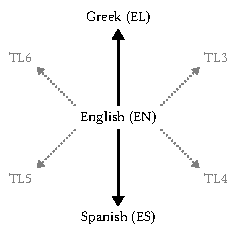
\includegraphics{./figures/4-1-starlayout.pdf}
\caption{The “star” layout of the study corpus} \label{fig:2:1}
\end{figure}

Concerning the description of the corpus contents, the following metadata has been used (based on the \textsc{tei} guidelines):

\begin{itemize}
\item for files (in the file header section): the audio and video file name/path, the film title, the publication statement (information concerning the distribution of the text);
\item for utterances: information on the speaker (e.g., \textsc{spk1} [Danny]), the time-stamp (\textit{anchorsynch}), and the dependent/aligned tiers with the Greek and Spanish translations respectively (\textit{spanGrp} type).
\end{itemize}

An example of an \textsc{xml}-tagged utterance and of its translations into \textsc{el} and \textsc{es}, as outputted from \textsc{elan} following processing in \textsc{tei}-\textsc{D}rop, is in \figref{fig:2:2}.

\begin{figure}
\caption{Example of an \textsc{xml}-tagged utterance} \label{fig:2:2}
\begin{lstlisting}
<div>
<u who="\# SPK1">
<anchor synch="\# T3497"/>
"We are not enemies, but friends.
<anchor synch="\# T3498"/>
</u>
<spanGrp type="subtitles el">
<span to="\#T 3498" from="\# T3497">"Δεν είμαστε εχθροί, αλλά φίλοι.</span> </spanGrp>
<spanGrp type="subtitles es">
<span to="\#T 3498" from="\# T3497">"No somos enemigos, sino amigos.</span> </spanGrp>
</div>
\end{lstlisting}
\end{figure}


\textsc{elan} is used to visualise each utterance in its context, together with the speaker and the aligned subtitled utterances.

\begin{figure}
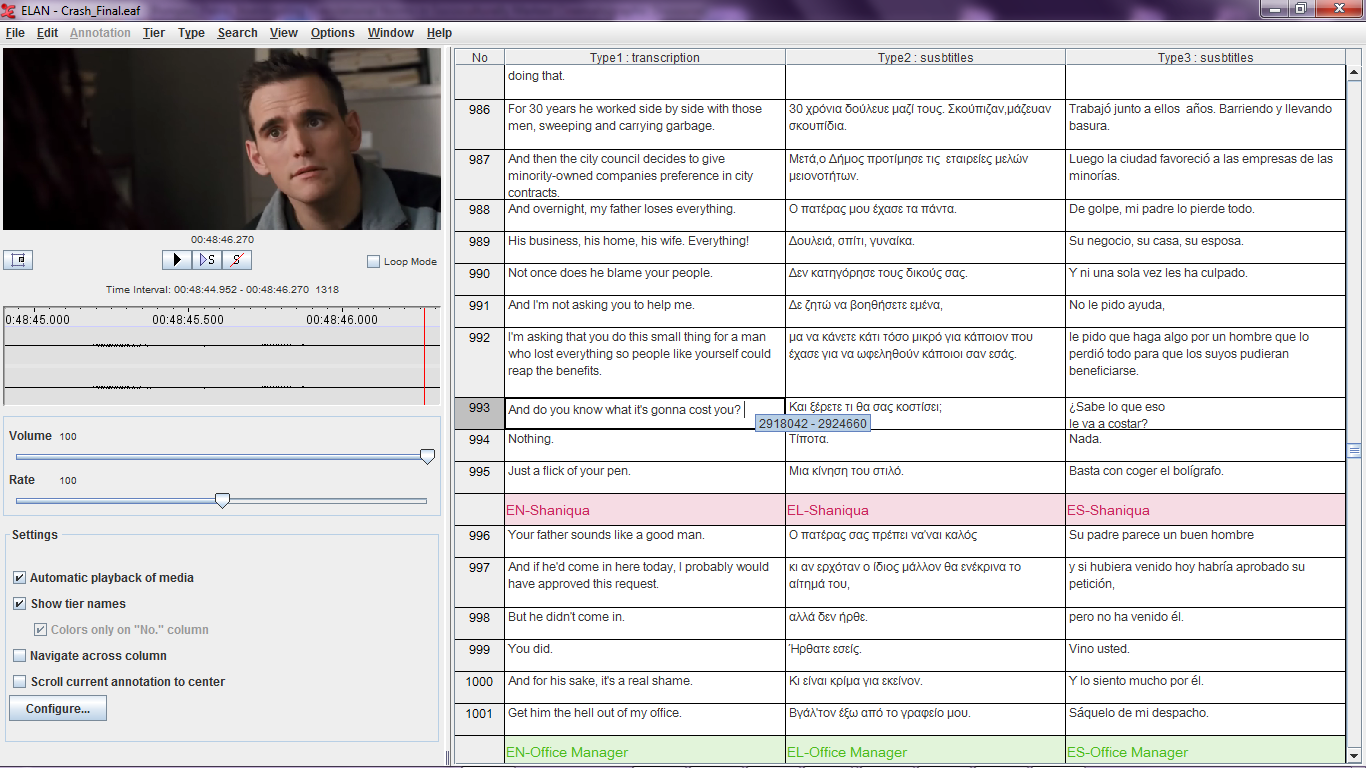
\includegraphics[width=1.0\textwidth]{./figures/4-2.png}
\caption{\textsc{elan} interface, in transcription mode}
\end{figure}

To manually annotate the corpus, we have used the \textsc{gate} platform \citep{Cunningham2002}.\footnote{The annotation methodology and a preliminary annotation scheme (regarding emotions) were first presented in \citet{Mouka2012}. The annotation scheme used in this paper was later finalised and has been reported in \citet{Mouka2014}.} The annotation was performed on the level of text chunks, i.e. of extended units of meaning \citep{Sinclair1996a}. \textsc{gate} is optimally designed for linguistic annotation. Even though \textsc{elan} can also be used for linguistic annotation, it would not be adequate for processing multiple speakers' conversations. \textsc{elan} has been primarily developed for psycholinguistic research and each layer of annotation depends on the principal layer attributed to a single speaker. This would be impracticable in the case of our corpus. The change of tool has made impossible the direct access to the audiovisual material and necessitated the simultaneous use of both platforms.

\subsection{Reference corpora} \label{sec:2:3:3}

Although the context of situation provides the main clues on how/why words are used in a specific utterance and what was really meant by it, it cannot be reasonably argued that there is one and only one meaning in each utterance, or a single and precisely determined stance, nor that such meaning or stance can be fully and indisputably perceived and decoded by the analyst. This also applies to our effort to distinguish racist-oriented from neutral discourse elements. What one considers as being blatantly racist or has “labelled” as politically incorrect may be considered “neutral” by others. While well-known racial slurs, such as the lexeme \textit{nigger}, are marked as offensive in all contemporary dictionaries, it can be observed that some of these terms used to be neutral in the past. In order to avoid -- as far as possible -- being influenced by preconceptions and personal beliefs, especially in view of the cross-linguistic nature of the investigation, the interpretation of how racist markers are used in discourse was based on the evidence provided by reference corpora, one for each of the three languages considered.\footnote{“Reference corpora [...] can be used as benchmarks for special corpora. Whenever we do not want to look at standard language as a whole but at some special phenomenon we happen to be interested in, we usually have to compile a corpus that fits our research focus” \citep[68]{Teubert2007}. In Translation Studies, the use of reference corpora as discourse benchmarks is exemplified, \textit{inter alia}, in \citet[516]{Kenny1998}.}

In the comparative analysis the intuition of the annotator was supplemented with the interpretation of data from the corpora pre-loaded on the SketchEngine platform \citep{Kilgarriff2004}.\footnote{\url{www.sketchengine.co.uk}.} These corpora are: enTenTen12 (11+ billion words), GkWaC (124 million words) and esTenTen11 (2.1 billion words), respectively for English, Greek and Spanish.\footnote{For a definition of the TenTen collection of corpora, see \citet{ Jakubicek2013}.} The selected corpora offer texts collected from the Web and, as such, include a variety of text genres and a variety of language uses (both formal and informal). Furthermore, the SketchEngine system allows the visualisation of an extended co-text of concordances. Web corpora also include authentic texts that have not been stylistically filtered and can thus present higher frequencies of informal language, slang and insulting words compared to other general reference corpora (e.g., in the case of Greek, the Corpus of Greek Texts/\textsc{sek}\footnote{\textsc{sek} is provided by the University of Athens \url{http://sek.edu.gr}.} and the Hellenic National Corpus/\textsc{hnc}\footnote{\textsc{hnc} is provided by the Institute for Language and Speech Processing (\textsc{ilsp}) \url{http://hnc.ilsp.gr}.}), which usually comprise only authoritative texts or texts that have previously been published in printed form or broadcast and, in that sense, have undergone pre-print editing and perhaps been subjected to cultural and linguistic “filtering” prior to their publication. In most cases, the content of such general reference corpora is “mainstream”/standard texts.\footnote{\citet[65--66]{Teubert2007}, referring to English, define its “standard” form as corresponding to the “private annual reading load of educated middle class citizens” and go on to describe a possible formulation of this definition, in corpus design terms. Such an analogy could also be made for Greek, even though it is not always clear or substantiated how the textual sub-categories would be included in such a corpus.}

\section{Corpus annotation: Analysis and examples} \label{sec:2:4} 
\subsection{Implementing the Appraisal Theory} \label{sec:2:4:1}

This study focuses on the “negative” expressions of racism, i.e., on the discoursal emphasis on negative and/or de-emphasis of positive “things” about \textit{Them}, of which there are many in the corpus. It is beyond our scope to examine the emphasis on positive things and/or the de-emphasis of negative things about \textit{Us}, although these are, more often than not, the other side of the same coin \citep[44]{Dijk2000b}.

For the purposes of our work we have partially adapted the Appraisal Theory model by focusing on the classification and “graduation” of attitudes, including the graduation of engagement features, which are labelled “strength” in our schema. Thus, strength is linked to:

\begin{itemize}
\item the valence of an evaluation and its intensification/mitigation; and
\item the intensity of the speaker's engagement with the evaluation, given that our focus is on the degree of the negative attitude expressed by the speaker as a whole.
\end{itemize}

The attitude types used are summarised as follows:
\begin{itemize}
\item \textit{Affect}: emotions and emotional reactions;
\item \textit{Judgement}: evaluation of behaviours;
\item \textit{Appreciation}: evaluation of phenomena, including aesthetics.
\end{itemize}

Our main focus is therefore on exploring the interpersonal nature, the tenor of the discourse and the social relations of the characters of the films, as far as racist stances are manifested in discourse, elements of which are the evaluation of behaviours and situations and the expression of negative emotions and opinions \citep[see][]{Fotopoulou2009}. In this sense, we have categorised and manually annotated “[a]ttitudes [...] divided into three regions of feeling, ‘affect’, ‘appreciation’ and ‘judgement’” \citep[35--43]{MartinWhite2005}. 

For the purposes of our analysis, we annotated every segment of racist attitude of the film characters (appraisers) that express negative evaluations towards a person or a group of another ethnicity/“race”/religion (appraised entity). All candidate instances are interpreted and classified as instantiations of a type of attitude towards “Others”. In this sense, the utterance \textit{Minorities don't give two shits about this country} (American History X), taken semantically, simply informs us about the indifference (affect) of minorities towards \textit{this country}. However, considering how it is used in the given context, we focus on the interlocutor’s intended meaning, which is to implicitly criticise the members of minorities as indifferent free-loaders who just want to exploit the country. Therefore, it is annotated as an implicit judgement.

\subsection{Attitude types and usage perspective} \label{sec:2:4:2}

A systematic classification of racist attitudes requires the clearest possible definition for each category, since the boundaries among attitude types are not always accurate and undoubted. This is not surprising, given that “[i]n a general sense, affect, judgement, and appreciation all encode feeling” \citep[147]{Martin2000}. It cannot be argued that negative judgements or appreciations bear no traces/nuances of affect and that speakers can either express emotions or judge. As a matter of fact, “[a]ffect can perhaps be taken as the basic system […]” (ibid.), as an immanent or emerging characteristic of every attitude. Through this perspective, “[a]s judgement, affect is re-contextualised as an evaluation matrix for behaviour [...] [a]s appreciation, affect is re-contextualised as an evaluation matrix for the products of behaviour (and wonders of nature)” \citep[147]{Martin2000}.

In this sense, we have annotated as instances of \textit{affect} all expressions of emotions, as signs of emotional reactions of the characters related to the specific discourse type. Further, \textit{appreciation} was defined as evaluations, mainly aesthetic, of humans as entities, as evaluations not related to their behaviour but to their characteristics such as colour, ethnicity, religion, physical characteristics and supposed inherent characteristics. Such assessments are negative markers of difference. Finally, \textit{judgement} which “deals with attitudes towards behaviour, which we admire or criticise, praise or condemn” \citep[42]{MartinWhite2005} applies to cases that can be defined as rationalisations of a fact or as reflecting a causal relation between things or facts. On the contrary, in \textit{appreciation}, the speaker's stance is intuitive or dogmatic, i.e. non-refutable in the specific context of situation. In our opinion, this formalisation defines more objectively the classification of attitudes compared to the broader and more inclusive definition offered by \citet[42--45]{MartinWhite2005}.

The basic tri-fold categorisation of attitude as applied in this study is as follows:

\begin{itemize}
\item \textit{Affect}: characterises negative emotions and emotional reactions towards Others, principally instances that are indicative of hate and anger based on or evoked by racial/ethnic/religious differences.
\item \textit{Appreciation}: characterises negative evaluations of Others based on their inherent characteristics, or on characteristics that are presented as such, dogmatically used as sufficient reasons for negative evaluations.
\item \textit{Judgement}: characterises negative evaluations of the behaviour of Others, judged as people that act in relation to their racial/ethnic/religious difference.
\end{itemize}

In the paragraphs below, these types are exemplified.

\subsubsection{Affect}

\ea \label{ex:2:1} Your mother, she \emph{hated them niggers} too (\textit{Monster's Ball})
\z
\ea \label{ex:2:2} That means \emph{not welcome} (\textit{American History X}) [utterance addressed to a Jew while the speaker reveals his swastika tattoo]
\z
\ea \label{ex:2:3} Take your fucking pizza piece and \emph{go the fuck back to Africa} (\textit{Do the Right Thing})
\z
\ea \label{ex:2:4} Yeah, \emph{fuck off, you Paki bastards} (\textit{This is England})
\z
\ea \label{ex:2:5} \emph{What the hell are those niggers} doing out there? (\textit{Monster's Ball})
\z

\subsubsection{Appreciation}

\ea \label{ex:2:6} We'll let the \emph{niggers, kikes and spics} grab for their piece of the pie (\textit{American History X})
\z
\ea \label{ex:2:7} A \textit{bunch of people} who \emph{aren't even citizens of this country} [{\dots}] (\textit{American History X})
\z
\ea \label{ex:2:8} She \emph{smells like fish and chips and guacamole} (\textit{American History X})
\z
\ea \label{ex:2:9} Three and a half million of us, who can't find fucking work because \emph{they're taking them all, because it's fucking cheap labour} (\textit{American History X})
\z
\ea \label{ex:2:10} How come \emph{niggers are so stupid}? (\textit{Do the Right Thing})
\z
\ea \label{ex:2:11} Magic, Eddie, Prince, are not \emph{niggers}. I mean, they're not \emph{black}, I mean... (\textit{Do the Right Thing})
\z

\subsubsection{Judgement}


\ea \label{ex:2:12} Look at these little \emph{fucking sewer rats} (\textit{This is England}) [referring to young immigrants playing in a yard]
\z
\ea \label{ex:2:13} \emph{Immigration, \textsc{aids}, welfare, those are problems of the black community, the Hispanic community, the Asian community} (\textit{American History X})
\z
\ea \label{ex:2:14} One in every three black males is in some phase of the correctional system. Is that a coincidence or do these people \emph{have like a racial commitment to crime}? (\textit{American History X})
\z
\ea \label{ex:2:15} All right. Well, you know what I can't do? I can't look at you without thinking about the \emph{five or six more qualified white men who didn't get your job} (\textit{Crash})
\z
\ea \label{ex:2:16} He's one of those \emph{proud to be nigger people} (\textit{American History X})
\z

Although “interpersonal epithets” \citep[see][376--377]{Halliday2014}, e.g. evaluative adjectives, are the most obvious evaluative device of language, the lexico-grammatical choices that express attitude are infinite, especially if we consider that evaluative uses of language can be present in discourse both explicitly and implicitly \citep[see][23] {Munday2012}. As shown in the above examples, the lexico-grammatical means to express attitude are vast and not limited to closed semantic or grammatical categories.

In addition, phenomena investigated from another point of view in previous studies are also evident in our data, but are further analysed as instantiations of evaluative attitudes. Referential/nomination strategies and predication strategies, such as racial slurs and metaphors (\textit{sewer rats}) analysed by \citet{Reisigl2001} as a means to categorise membership, are analysed here as evidences of the speaker's stance. Thus, we observe the presence of racial slurs, such as \textit{nigger}, in all three types of attitude:

\begin{itemize}
\item used to express mere anger and hate, as in \REF{ex:2:1} and \REF{ex:2:5},
\item used in appreciations just to refer to Others in a disparaging manner, presenting the fact of belonging to other racial groups and/or having their “inherent” characteristics as being \textit{per se} negative, as in \REF{ex:2:6} and \REF{ex:2:11}, or
\item used in judgements to negatively evaluate a certain person's behaviour, which is presented as related to the fact that he/she is black \REF{ex:2:12}.
\end{itemize}

The interpretation of each instance is based on the context of situation, and is further based on the presence of various markers, either explicitly stated, as in \REF{ex:2:1} where the verb \textit{hate} is used, or using interjections such as \textit{go the fuckback}, \textit{fuck off} and \textit{what the hell} [in \REF{ex:2:3}, \REF{ex:2:4}, and \REF{ex:2:5}].

On the other hand, in \REF{ex:2:6} racial slurs are used instead of “neutral” ethnic denominations as disparaging terms, simply to mark the inferiority of the mentioned groups. The utterance in example \REF{ex:2:11} is a response to the interlocutor's argument that, despite his constant negative attitude towards black people, all his favourite celebrities (Eddie Murphy, Magic Johnson and Prince) are black. It is a representative example of how a highly marked racial slur is used as a negative appreciation, to evaluate people as being “nice” or “bad”.

Accordingly, our data includes many convictions and stereotyped visions of Others \REF{ex:2:7} and recurrent topics or \textit{topoi}, as “common-sense reasoning [that is] typical for specific issues” (\citealt{Dijk2000c} in \citealt[299, note 21]{BakerGabrielatos2008}; \citealt[see also][74–76]{Reisigl2001}). Examples are the \textit{topos} of finance \REF{ex:2:9}, the \textit{topos} of threat (\ref{ex:2:13}, \ref{ex:2:14}) and the \textit{topos} of justice or equal opportunities \REF{ex:2:15}. Such visions can be used as appreciations or judgements, i.e. presented as either negative phenomena, as in \REF{ex:2:9}, or as criticism of the behaviour of Others, as in \REF{ex:2:13}, \REF{ex:2:14} and \REF{ex:2:15}.


\subsubsection{Type overlaps}

As mentioned already, it is normal that the boundaries between categories are not always clear-cut: thus, in cases that could belong to more than one category, we have used double annotation: this is both methodologically permissible and of course technically possible. This allows for a subsequent analysis on both levels, e.g. of \textit{affect} and \textit{appreciation}, for the sake of contrastive analysis within the two categories, and hence for further refining the classification/annotation scheme.\newline

\ea \label{ex:2:17} You \emph{gold-teeth, gold-chain-wearing, fried-chicken and biscuit-eating monkey, ape, baboon, big-thigh, fast running, high-jumping, spear chucking, 360-degree basketball-dunking, titsoon, spade, moulignon}!
\z

In this sense, according to our definition of attitudes, the utterance in \REF{ex:2:17} used by an Italian-American in an aggressive manner to express hatred directed to a black person, shows negative affect. At the same time, the long list of epithets enumerated represent appreciations referring to his interlocutor.

\subsection{\textit{Attitude features}} \label{sec:2:4:3}

Attitudes are also analysed in terms of their features.

\subsubsection{Implicit and explicit attitudes} 

As mentioned above, we always categorise attitudes expressed towards persons or groups of other ethnicities/“races”/religions. In many cases, attitudes are not explicitly stated in the text, but evoked, expressed implicitly. Such an interpretation can rely on common knowledge, on the co-text and on the context of the situation.

\begin{quote}
“If by expressing meaning A, language users (also) mean B, such an implication can be reconstructed by recipients only on the basis of inferences from culturally shared knowledge of language meanings (e.g. as represented in the lexicon of the language) or more generally on the basis of shared knowledge, including particular knowledge about the knowledge of the speaker” \citep[168]{Dijk1995}.
\end{quote}

Thus, in example \REF{ex:2:8} above, one should know that \textit{fish and chips and guacamole} refer to the culinary traditions of Latin Americans in order to properly interpret it, whereas in example \REF{ex:2:12} knowledge about the policies of affirmative action against racial discrimination in the \textsc{usa} is crucial in order to interpret the utterance correctly. Moreover, in example \REF{ex:2:12} the term \textit{sewer rat} is used metaphorically to designate useless people that cause problems to society.

\subsubsection{Irony}

Irony is also a case of implicit meaning, a pragmatic phenomenon used to express a meaning contrary or different to the literal one. Once again, its recognition depends on the situational context which indicates something different than the apparent meaning of the utterance, the speaker's tone of voice or the “interpreters' assumptions about the beliefs or values of the text producer”  \citep[123]{Fairclough1992}. For instance, the utterance in example 18 is used to depreciate African-American literature:

\ea \label{ex:2:18} What is it, Black History Month? (\textit{American History X})
\z

\subsubsection{Indirect/Direct attitudes}
Some utterances do not express a racist attitude but are still indicative of the social roles of the participants and can reflect racism as internalised.\footnote{\textit{Internalised racism} is defined as the situation in which individuals, groups and cultures that have been subjected to racism and oppression, shift this racism to oppress themselves and others who have experienced racism and discrimination \citep[92]{Lawrence2002}.} These are cases where speakers comment the racist stance of others and are annotated as indirect references to racist attitudes.\newline

\ea \label{ex:2:19} Man's singing about lynching niggers. “Gonna buy me a rope and lynch me a nigger” (\textit{Crash})
\z
\ea \label{ex:2:20} Your partner's a racist prick (\textit{Crash})
\z

\subsubsection{Polarity}
Polarity refers to the positive or negative dimension of an attitude, distinguishing positive from negative affect, appreciation or judgement. As mentioned already, for the aims of our study we focus on negative instances.

\subsubsection{Strength} 
The strength of each instance is taken into account and an indication of low, medium or high valence is given to each instance. Admittedly, this is the most subjective parameter of our effort, so that in order to decide on the strength of an utterance inter-subjective agreement among the annotators was required in most cases. The collocational behaviour of the lexemes examined was assessed with the help of the English reference corpus.

\subsection{Annotation scheme overview} \label{sec:2:4:4}
The attitude classification outlined above and used as annotation scheme in the reported project can be schematised in \figref{fig:2:4}.

\begin{figure}
% 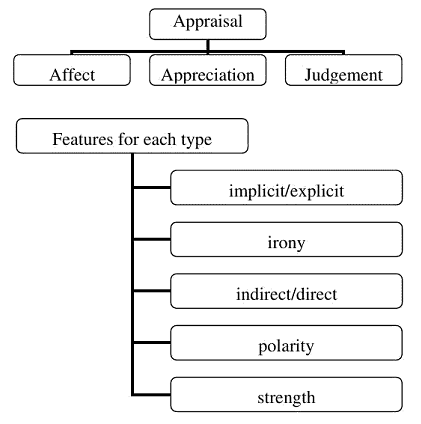
\includegraphics[width=.6\textwidth]{./figures/4-3.png} 
%4-3-Corpus-Annotation-Scheme.tex
\begin{tikzpicture}
[every rectangle node/.style={inner sep=6pt, rounded corners=5, draw}]


\node at (0,0) [rectangle] (appraisal) {Appraisal};
\node [below=5mm of appraisal, rectangle] (appreciation) {Appreciation};
\node [right=20mm of appreciation.east, rectangle] (judgement) {Jugdement};
\node [left=20mm of appreciation.west, rectangle] (affect) {Affect};

\draw [thick] (node cs:name=appraisal, anchor=south) -| (node cs:name=appreciation);
\draw [thick] (node cs:name=affect, anchor=north) |- +(0,.275) -| (node cs:name=judgement);


\node [below right=10mm and 0mm of affect.west, rectangle, text width=40mm, align=center] (features) {Features for each type}; 
\node [below right=4mm and 10mm of features.south, rectangle, text width=40mm, align=center] (implicit) {implicit/explicit};
\node [below=4mm of implicit, rectangle, text width=40mm, align=center] (irony) {irony};
\node [below=4mm of irony, rectangle, text width=40mm, align=center] (indirect) {indirect/direct};
\node [below=4mm of indirect, rectangle, text width=40mm, align=center] (polarity) {polarity};
\node [below=4mm of polarity, rectangle, text width=40mm, align=center] (strength) {strength};

\draw [thick] (node cs:name=features, anchor=south) |- (node cs:name=implicit);
\draw [thick] (node cs:name=features, anchor=south) |- (node cs:name=irony);
\draw [thick] (node cs:name=features, anchor=south) |- (node cs:name=indirect);
\draw [thick] (node cs:name=features, anchor=south) |- (node cs:name=polarity);
\draw [thick] (node cs:name=features, anchor=south) |- (node cs:name=strength);

\end{tikzpicture}
\caption{Corpus annotation scheme} \label{fig:2:4} 
\end{figure}

\section{Register shifts: Analysis and examples} \label{sec:2:5}

This study investigates how racist/heterophobic discourse is transferred when a film is translated into socio-cognitively distinct and somewhat remote linguistic systems. It tries to systematise changes of tenor \citep{Halliday1978} in translation by means of a comprehensive classification of attitudes and their cross-linguistic mapping.

We therefore believe that retrodictively \citep{Wright1971,Chesterman2008} the diachronic study of discourse features, and more generally of racism, in translation could also benefit from such a hermeneutic approach. In the examples below, the shifts observed in discourse transfer have been explained in the light of the relationship between participants in discourse.

\subsection{Examples} \label{sec:2:5:1} 
(\textit{Examples 21--24 are sourced from American History X; examples 25-27 are sourced from Crash.})

\ea \label{ex:2:21}
\begin{xlist}
\exi{}[\textbf{[\textsc{en}]}]{And now some fucking Korean owns it who fired \emph{these guys} and is making a killing because he hired \emph{40 fucking border jumpers}}
\exi{}[\textbf{[\textsc{el}]}]{Τώρα το 'χει ένας Κορεάτης, που απέλυσε τους \emph{δικούς μας} και θησαυρίζει επειδή προσέλαβε \emph{λαθρομετανάστες}}
\exi{}[\textbf{[Back translation]}]{Now a Korean owns it who fired \emph{our guys }and is making a killing because he hired \emph{illegal immigrants}}
\end{xlist}
\z

Derek, a young skinhead, gives a speech to the rest of the gang members, trying to convince them to attack a supermarket owned by immigrants. Throughout his speech, negative attitudes towards immigrants are abundant. Among other arguments, he uses a variety of \textit{topoi} as in, e.g. \textit{immigrants take our jobs}. He uses rather colloquial expressions and the register of his speech is highly informal, indicative of the brotherhood relations among the in-groups. In terms of Appraisal Theory, this utterance is considered to be a highly marked negative judgement about immigrants.

If we concentrate on the last part of the utterance, that is \textit{40 fucking border jumpers} and its respective Greek version rendered as\textit{ λαθρομετανάστες}, we notice immediately that the strength of the judgement is significantly altered. A closer look at each component of the \textsc{tl} unit of meaning reveals that \textit{border jumper}, an apparently neutral term describing an action, is used as a depreciative, non-fixed, and possibly colloquial, synecdoche of \textit{immigrants of Hispanic/Mexican origin}. An analysis of the term in enTenTen12 has returned only 57 hits of \textit{border jumper(s)}, i.e. a negligible frequency in the enTenTen12 corpus (0.0 per million). Furthermore, as an analysis of the concordance lines reveals (see \figref{fig:2:5}, below), the term is used almost exclusively in a negative and highly disparaging sense (\textit{border jumpers want our wealth}; \textit{drug smugglers}, \textit{human traffickers}, \textit{border jumpers and other assorted criminals}; \textit{border jumpers are slapping those legal immigrants}). Moreover, the presence of \textit{fucking} (in the cluster \textit{fucking border jumpers}), as an intensifier, as well as the emphatic mention to the number of immigrants employed, reinforce the overall negative prosody of the judgement, making it highly negative. On the other hand, the Greek translation of the utterance is limited to \textit{λαθρομετανάστες} [clandestine immigrants], which is a generic term with no real connotation about the specific origin of the immigrants in question. By contrast, in GkWaC, the term \textit{λαθρομετανάστης} has a frequency of 5.9 per million and its “ideologically neutral” synonym \textit{παράνομος μετανάστης}\footnote{The use of the prefix “λαθρο-” (a derivative of the adjective \textit{λαθραίος} {clandestine, smuggled}) to designate economic or political immigrants has been criticised by human rights and political organisations as being negatively loaded, even though this is not always the case, since language economy, not surprisingly, seems to opt for the single-word designator (\textit{λαθρομετανάστης}) rather than for the presumably more neutral two-word unit (\textit{παράνομοςμετανάστης}). This is apparent also in the concordances derived from GkWaC, where most occurrences do not have a negative connotation. The neutral (and hence stabilised as politically correct) designator \textit{παράνομος} (illegal) is used instead by the administration.} appears with a frequency of 0.7 per million. As to its usage profile, the term in question appears in various text genres and, most importantly, belongs to “standard” Greek as it is present in authoritative language.\footnote{See above, note 17.} The rendition of the utterance in Greek is a translation shift, in both field and tenor. The judgment loses its strength and maintains only the negative nuance inferred by the context of situation, as well as by the invented contrastive relation \citep[87--89]{Fairclough2003}, i.e. by the contrast between \textit{δικούς μας} `our guys' and \textit{λαθρομετανάστες} `illegal immigrants', that has been added explicitly in the \textsc{tt}.

\begin{figure}
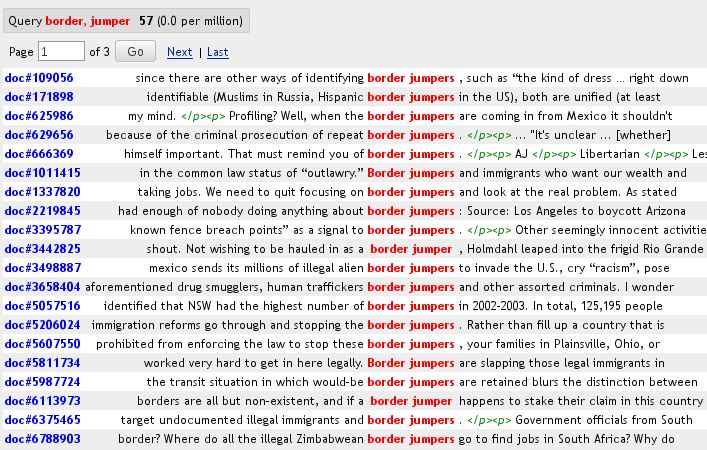
\includegraphics[width=.9\textwidth]{./figures/4-4.png}
\caption{Concordance lines, \textit{border jumpers}, GkWaC, in SketchEngine} \label{fig:2:5}
\end{figure}

\ea \label{ex:2:22}
\begin{xlist}
\exi{}[\textbf{[\textsc{en}]}]{I mean, Christ, Lincoln \emph{freed the slaves}, what, like hundred and thirty years ago. \emph{How long does it take to get your act together}?}
\exi{}[\textbf{[\textsc{el}]}]{Ο Λίνκολν \emph{απελευθέρωσε τους σκλάβους} πριν 130 χρόνια. \emph{Πόσον καιρό χρειάζεσαι για να γίνεις άνθρωπος;}}
\exi{}[\textbf{[Back translation]}]{Lincoln \emph{freed the slaves} a hundred and thirty years ago. How long does it take to become a human?}
\end{xlist}
\z

During a family dinner, Derek argues with his professor (who apparently has an affair with his mother) about riots in the black neighbourhoods. Example \REF{ex:2:22} comes to reinforce his argument that the sheer number of jailed black people proves their racial commitment to crime. The idiom used in this example, \textit{get one's act together}, has the meaning of getting organised and being on schedule. The utterance is implicitly ironic. In our study, the source segment has been noted as a negative judgement of medium strength, this being mainly due to the ironic nature of both the argument and the reference to the end of slavery. On the other hand, the Greek translation uses the idiom \textit{γίνομαι άνθρωπος} `become human' (GkWaC frequency: 1.9 per million) which has the meaning of “becoming an ethical and useful citizen”, thus implying a shift towards a stronger negative judgement about the social attitude of black people.\newline

\ea \label{ex:2:23}
\begin{xlist}
\exi{}[\textbf{[\textsc{en}]}]{We'll let the \emph{niggers, kikes and spics} grab for their piece of the pie.}
\exi{}[\textbf{[\textsc{es}]}]{Dejemos que \emph{negros y latinos} se lleven su parte.}
\exi{}[\textbf{[Back translation]}]{Let the \emph{blacks} and the \emph{Latinos} get their part.}
\end{xlist}
\z

The leader of the skinhead gang, a middle-aged male, tries to convince Derek that their organisation is going to stop being a small gang and will now grow into something very serious and powerful all over the country. He explains how he plans to act in order to achieve it.

In example \REF{ex:2:23} above, we mark the use of three racial slurs, \textit{nigger} (enTenTen12 frequency: 0.9 per million) as highly negative appreciations towards Jews, Latinos, and black people respectively. In the Spanish \textsc{tt}, the racial slurs of the original are shifted towards neutralisation (\textit{negros} and \textit{latinos}), while the reference to Jews (\textit{kikes}) is eliminated. In all, the negative appreciations that are inherent in racial slurs are eliminated. Although in Spanish there is a lexeme, \textit{negrata}, which has the same derogatory connotation as \textit{nigger}, translating \textit{nigger} as \textit{negro} is a recurrent practice in our corpus. However, \textit{negrata} is a term with a very low frequency (only 97 tokens in esTenTen11), while \textit{nigger} appears with a frequency of 0.9 per million in enTenTen12. This observation could be indicative of the reasons that made Spanish subtitlers opt for the neutral term, avoiding the use of an uncommon term. On the other hand, \textit{spic}, a term that could have been translated as \textit{sudaca} (a Spanish racial slur with presumably similar connotations with 431 tokens in esTenTen11) is also avoided. In both cases, the translator opts for neutralising the rendition of the original utterance.

\ea \label{ex:2:24}
\begin{xlist}
\exi{}[\textbf{[\textsc{en}]}]{Name your price, \emph{cracker}.}
\exi{}[\textbf{[\textsc{es}]}]{Di tu precio, \emph{blanco}.}
\exi{}[\textbf{[Back translation]}]{Name your price, white guy.}
\exi{}[\textbf{[\textsc{el}]}]{Πες το ποσόν, \emph{βλάχο}.}
\exi{}[\textbf{[Back translation]}]{Name your price, country bumpkin.}
\end{xlist}
\z

During a basketball game in the neighbourhood court, members of the skinhead gang start to quarrel with members of a “black gang”. Derek has a bet; he proposes a “whites against blacks” game. The answer in \REF{ex:2:24} comes from one of the opponents, indicating that they accept the bet.
In example \REF{ex:2:24} above, the disparaging term \textit{cracker} (showing negative appreciation, i.e. for a poor white person, usually from the South) is translated as \textit{blanco} `white' in Spanish, but as \textit{βλάχο} `country bumpkin' in Greek. In this case, the Spanish subtitler succeeds in maintaining the racial nuance of the term, although the strength of the negative appreciation is diminished, while the Greek subtitler eliminates the racial reference and only transfers the aggressive tone of the dialogue. 

\ea \label{ex:2:25}
\begin{xlist}
\exi{}[\textbf{[\textsc{en}]}]{- Do you speak English? - I am speaking English, you stupid cow!}
\exi{}[\textbf{[\textsc{el}]}]{- Θα μιλήσετε Αγγλικά; - Μιλάω Αγγλικά!}
\exi{}[\textbf{[Back translation]}]{- Are you going to speak English? - I speak English!}
\end{xlist}
\z

In example \REF{ex:2:25} above, an Asian woman enters a hospital screaming the name of her husband. The intuitive reaction of the nurse is to ask her if she speaks English, a reaction reflecting the stereotype that immigrants do not speak the language of the host country. Thus, we mark this instance as a low strength negative appreciation, yet expressed in a polite manner. The Greek subtitler opts for a more aggressive-impolite way in rendering this question, \textit{θα μιλήσετε Αγγλικά} `Are you going to speak English?' strengthening the negative valence of the utterance. There are many similar examples in our corpus, pointing to the linguistic identity as a marker of difference. \citet[111]{Sella2001} argues that language is involved in matters of political and social texture, by functioning as the defining element of the nature of multiple human groupings, either positively by delineating “Us”, or negatively, by excluding allophones from the said group: in this case, the interlocutors are self-determined contrastingly, both within and outside a linguistic group (the “Others”).

\ea \label{ex:2:26}
\begin{xlist}
\exi{}[\textbf{[\textsc{en}]}]{Stupid \emph{wetback}}
\exi{}[\textbf{[\textsc{es}]}]{Estúpida \emph{sin papeles}}
\exi{}[\textbf{[Back translation]}]{Stupid undocumented immigrant}
\end{xlist}
\z

In \REF{ex:2:26}, an Asian and a Latin American woman are involved in a car crash. While they quarrel, the first one calls the other a \textit{wetback}. The term is highly disparaging and refers to illegal Latin Americans (especially Mexicans) as a descriptor of the way Mexicans enter the US by crossing the Rio Grande. Therefore, it has been marked as a negative judgement utterance. Although the term is decades-old and has been used even in the title of a deportation programme of the US in 1954 (the so-called “Operation Wetback”, see \citealt{Hernandez2006}), today it is used in a highly derogatory manner as a racial slur. As shown in \figref{fig:2:6}, the most significant collocations of wetback (sorted by Mutual-Information, in a query window of {-10 to +10} tokens) are other racial slurs, especially in their context of usage (e.g. \textit{mojado}, \textit{beaners}, \textit{spics}, \textit{kike}, \textit{nigger}, \textit{chink}, \textit{greaser}, \textit{lowlife}, etc.).

\begin{figure}
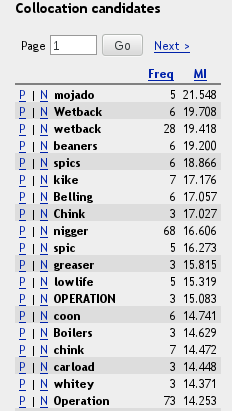
\includegraphics[width=.3\textwidth]{./figures/4-5.png}
\caption{Collocates of \emph{wetback} in enTenTen12, sorted by Mutual Information (\textsc{mi}) in SketchEngine} \label{fig:2:6}
\end{figure}

On the other hand, the Spanish translation uses \textit{sin papeles} `undocumented immigrants'. This is a rather neutral term to refer to illegal immigrants. In esTenTen11, the most significant collocates of \textit{sin papeles} (see \figref{fig:2:7}) are emotionally neutral (\textit{inmigrante} `immigrants', \textit{empadronar}/\textit{empadronamiento} `inclusion in the town registry', \textit{redadas} `raids', \textit{patera}/\textit{pateras} `dinghy') and an analysis of the concordances shows that the term is used also in texts, in support of the human rights of immigrants.

\begin{figure}
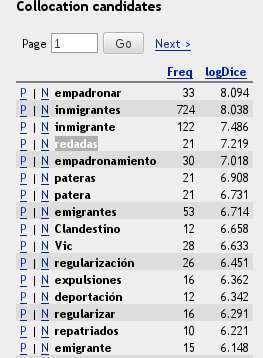
\includegraphics[width=.4\textwidth]{./figures/4-6.png}
\caption{Collocates of \emph{sin papeles} in esTenTen11, sorted by logDice in SketchEngine} \label{fig:2:7}
\end{figure}

In other words, the racist tone of the insult, even though it is still present in the Spanish text, is reduced in the interpersonal component of the utterance.

\ea \label{ex:2:27}
\begin{xlist}
\exi{}[\textbf{[\textsc{en}]}]{- You wanna buy these Chinamen? - Don't be ignorant. They're Thai or Cambodian. Entirely different kind of \emph{chinks}.}
\exi{}[\textbf{[\textsc{es}]}]{- ¿Vas a comprar esos chinos? - No seas ignorante. Serán tailandeses o camboyanos. Son unos \emph{amarillos} distintos.}
\exi{}[\textbf{[Back translation]}]{Should be Thai or Cambodian. They are different yellow people.}
\end{xlist}
\z

Once again, a character of \textit{Crash} uses a racial slur to refer to a group of Asians. He, quite ironically, has just decided to set them free instead of accepting money to “sell” them with the truck he robbed and proved to have been used for human trafficking. This is a negative appreciation texteme. Once again, \textit{chink} (queried in SketchEngine as a noun) was found to collocate with other racial slurs in our reference corpus. However, a similar query for \textit{amarillo} `yellow' does not yield any results, since as a noun it refers also to the colour, and in the tool used, semantic disambiguation is not possible. However, the use of a colour to designate a race does not necessarily indicate a racist stance, given that the utterance is not directed at Asians. This explanation is consistent with the definition of \textit{amarillo}, taken from the online version of the \textit{Diccionario de la Real Academia Española} \textit{(\textsc{drae})}, which is not marked as derogatory, but as simply referring to the Asian race.\footnote{“Dicho de un individuo o de la raza a que pertenece: De piel amarillenta y ojos oblicuos. Apl. a pers., u.t.c.s.” \url{http://goo.gl/oelvVZ}.}


\subsection{Summary of findings} \label{sec:2:5:2}
Each language/culture produces and stabilises forms of expressing (racist) meanings that are unknown or at least asymmetrically\footnote{For a discussion on cultural asymmetry in translation, a concept coined in \textsc{ts} by \citet{EvenZohar2005}, see e.g. \citet{Klaudy2012}.} represented in other languages and cultures. Racial slurs are a clear example of this and constitute crucial points for the translator, who often mitigates or omits them. Even though the mitigation of racial slurs is the general tendency in our corpus, there are also cases of over-toning of racist attitudes, e.g. in examples \REF{ex:2:22} and \REF{ex:2:25}; in both these examples, the (racist-oriented) interpersonal meaning is intensified in the \textsc{tl}, though both target utterances lack marked epithets (slurs). Such instances should be explored further. This article has discussed different types of register shifts, without attempting to provide a systematic analysis (for instance, we did not consider the many instances of racist discourse which did not undergo significant register shift in translation). Such a systematic analysis, which shall be pursued in further research, will hopefully provide a more “sustainable” picture of how racist discourse is handled in translation.

\section{Conclusions} \label{sec:2:6}

This paper has presented a research, based on the PhD thesis of the first author, aimed at investigating the translation of racist discourse in Anglophone films subtitled in Greek and Spanish.

To this end, we have developed a linguistic annotation model in order to systematically categorise racism-related utterances in original films and in their subtitled versions. Instances of stereotyped views, prejudices, racist attitudes and emotions triggered by racism were coded using an annotation scheme based on Appraisal Theory.

The reference corpora used for the analysis were extremely useful, though with some limitations. Firstly, they were neither corpora of spoken discourse nor balanced corpora. Secondly, some of the terms looked up have very low frequencies and therefore do not allow for a safe description. Thirdly, it was not possible to find reliable evidence for ambiguous terms such as \textit{amarillo} or \textit{sin papeles}. In many cases the meaning of a racist expression could be interpreted only by analysing its context in the film.

Our analysis of register shifts in translation, based on a Systemic Functional Linguistic approach, is promising for the descriptive study of the socio-culturally marked discourse of racism and aims to serve as an explanatory basis for addressing broader questions:

\begin{itemize}
\item Is it possible, and if so how, to refine the definitions of heterophobia that have formed part of our initial motivation in functional linguistic terms?
\item Which is the relation between cinema and socio-linguistic reality in the perception of xenophobia?
\item What are the implications of such an analysis, in relation to the comprehension of racist discourse and its root causes in the modern Greek and European linguistic and cultural reality?
\end{itemize}

Last but not least, our findings so far point to the assumption that such an approach could, indeed, be linked systematically to the critical study of the role of translation in the diachronic development of the sociolinguistic dimension of racism.

\printbibliography[heading=subbibliography,notkeyword=this]

\end{document}
%\documentclass[output=paper]{LSP/langsci}
\author{Naroa Zubillaga, Zuriñe Sanz and Ibon Uribarri}
\title{Building a trilingual parallel corpus to analyse literary translations from {German into Basque}}
%\epigram{Change epigram in chapters/01.tex or remove it there}
\abstract{The aim of this paper is to present the steps we undertook to build our multilingual-aligned parallel corpus created to analyse translations from German into Basque and to report initial results. Translation into Basque is a quite complex phenomenon, and this complexity is reflected in the design of the corpus. When carrying out research into literary translations from German into Basque, we deal with direct translations from German into Basque, but also with indirect translations through Spanish versions. In order to observe both texts in the case of direct translations and all three texts for indirect translations, we have created an aligned, parallel, trilingual corpus. We have also created a search engine which is linked to the corpus. This allows for easy queries and obtains results from both direct and indirect translations. The research carried out with the corpora presented in this paper has revealed cases of standardisation and interference. Evidence for both of \citeauthor{Toury2012}'s (\citeyear{Toury2012}) translation laws are identified in direct as well as indirect translation.}
\maketitle
\rohead{\thechapter\hspace{0.5em}Building a trilingual parallel corpus} % Display short title
\begin{document}
\hyphenation{A-leus-ka-Phra-se-o}
\hyphenation{orgu-lloso}
\section{Introduction} \label{sec:3:1}
  
This paper looks at the process of creating a trilingual aligned parallel corpus which takes into account direct translations from German into Basque and indirect translations through Spanish versions. We also provide some examples to illustrate the application of this corpus in our ongoing research on German to Basque translation. Creating a multilingual corpus and using it as a tool in our research projects enables us to conduct a systematic work within Translation Studies. According to \citet[216]{Corpas2008}, in less than a decade all Translation Studies branches, and mainly the descriptive branch, have benefited from corpus linguistics. Studies that are based on well designed and organised corpora lead to a qualitative and quantitative development of the discipline.

\citet{Xiao2009} give an overview of \textsc{cbts} on the Holmes-Toury map \citep[243]{Xiao2009}. Since our approach is descriptive, we concentrate on the descriptive branch of Translation Studies mentioned above, leaving aside the applied and theoretical fields.

The research line initiated by \citet{Baker1993}, which focuses on the product, has generated most work in this area. Baker and her colleagues at the University of Manchester created the Translational English Corpus (\textsc{tec}) and many studies \citep[e.g.][]{Lavios1998b,Olohan2000,Olohan2003} made use of this corpus to search for translation universals. \citet[244]{Xiao2009} even state that “the majority of product-oriented translation studies attempt to uncover evidence to support or reject the so-called translation universal hypothesis”. Other scholars, such as \citet{Kenny2001}, acknowledge the value of monolingual translational corpora, but they also argue that these kinds of studies would benefit from corpora including source texts: “while monolingual translational corpora have been invaluable in attempts to describe the specific nature of translated text and to pinpoint aspects of the styles of individual translators (and not just original authors), some researchers (\citealt[565]{Lavios1998b}; \citealt[565]{Puurtinen1998}) have argued that studies based on them may sometimes need to be supplemented by an analysis of the relevant source texts” \citep[62]{Kenny2001}.

Another research line focuses on the process. These kinds of studies are usually based on parallel corpora which help the researcher compare source and target texts. \citet{Utka2004}, for example, based on an English--Lithuanian parallel corpus consisting of original European Community law texts and three draft versions (the first translator's draft, the intermediate version and the final translation) for each source text, reports cases of “normalization, systematic replacement of terminology and influence by the original language” \citep[246]{Xiao2009}. In reference to the development of such parallel corpora, \citet{Ji2010} mentions that, due to the costs and copyright issues, the most commonly used type of corpora is the “small-scale topic-specific parallel corpora” \citep[6]{Ji2010} and that “the usefulness of this type of \textsc{diy} corpus, when studied in conjunction with larger-scale comparable corpora, translational or non-translational, may be maximally extended” \citep[6]{Ji2010}.

\enlargethispage{1\baselineskip}
A third line of research, corpus based function-oriented descriptive studies, has been rather less explored “possibly because the marriage between corpora and this type of research, just like corpus-based discourse analysis \citep[e.g.][]{Baker2006}, is still in the `honeymoon' period” \citep[247]{Xiao2009}.

In our case, as lecturers and researchers in the area of Translation Studies at the University of the Basque Country (\textsc{upv}--\textsc{ehu}) working within the framework of the research group \textsc{tralima}/\textsc{itzulik}, we have set up a corpus-based translation study.\footnote{GIC 12\_197, IT728--13, UFI 11\_06, \textsc{upv}/\textsc{ehu}.} As we all teach translation courses (from German into Basque and Spanish), we are aware of the benefits a corpus could have for translation didactics. As researchers, on the other hand, our main goal is to look into how translations have been performed from German into Basque; that is, we want to examine translational behaviour. On the one hand, we compare the source text with the corresponding target text(s) based on a parallel corpus. In that sense, the study is process-oriented.\footnote{We are aware of the fact that there are other approaches to study translation process, such as think-aloud protocols (TAPs) or the translog system. However, our aim is to study the process at a textual level using the parallel corpus.} However, on the other hand, this research is also product-oriented, since we focus on the target texts and culture in order to explain certain translational phenomena. For this reason we make use of and refer to already existing Basque monolingual corpora, a field that has attracted the attention of Basque researchers since the 1980s.

The first Basque monolingual corpus was created in 1984, and although there was a considerable hiatus until the next corpus was created (2002), generally speaking, this field has been growing constantly. \textsc{etc} (EgungoTestuenCorpusa),\footnote{The corpus' website is: \url{http://www.ehu.es/etc/.}} which was made freely available in 2013, contains 204.9 million words and is the largest Basque monolingual corpus created to date. The Basque Institute of the University of the Basque Country has created a reference corpus balanced in terms of type of texts, proportion of original and translated texts, year of publication, and so on. \enlargethispage{1\baselineskip}

However, the use of corpora in the academic field of Basque Translation Studies is very recent. \citet{Barambones2012}, who analysed the translation into Basque of audio-visual products for children on Basque public television, did use a corpus, but conducted his study by manually arranging the source and target texts in a chart. \citet{Manterola2011} analysed translations of Basque literary works into other languages, focusing on translations of the Basque writer Bernardo Atxaga. She built a large multilingual digital parallel corpus with 12 original works in Basque and their translations into seven languages. She used WordSmith Tools \citep{Scott2004} to build and analyse her corpus, but encountered problems while aligning her corpus at sentence level and the result of alignment at paragraph level was quite unsatisfactory.

\section{The Aleuska corpus} \label{sec:3:2}

Taking both of these precedents into account, and since there was no existing corpus linking the languages we wanted to work with, we had to create our own corpus. The starting point was the Aleuska database, a catalogue of German to Basque translations which was started in 2003 and which has been supplemented in subsequent years by consulting different Basque as well as German bibliographical databases, such as the Index Translationum,\footnote{\url{http://portal.unesco.org/culture/en/ev.php-URL_ID=7810&URL_DO=DO_TOPIC&URL_SECTION=201.html}.} the Deutsche Nationalbibliothek\footnote{\url{http://www.dnb.de/DE/Home/home_node.html}.} or the database for the Network of Basque Public Libraries.\footnote{\url{http://www.katalogoak.euskadi.net/cgi-bin_q81a/abnetclop/O9406/ID0cbc23a1/NT1?ACC=111&LANG=en-US}.} We now have a catalogue of approximately 700 entries. In addition to the usual data for each entry of the catalogue, such as the original title, the author, the translator, the year of publication and the publisher, we also tried to indicate whether the translation was direct or indirect. The texts were classified either as direct or indirect translations based on peritextual as well as epitextual information. This is of interim value, as the assumed direct/indirect character or the translation has to be verified through a more detailed analysis of the texts in the corpus. The uncertain nature of the information about translation directness makes it appropriate to adopt the term “assumed translations”, a term proposed by \citet{Toury1995} for texts with an ambiguous translation status. Thus, by using the term “assumed direct/indirect translation”, we are expanding Toury's concept of “assumed translation” to the mode of translation. For instance, detailed analysis has shown that translations catalogued as direct at macro-level could contain traces of indirectness at micro-level. Since we needed to avoid absolute categories, the concepts of assumed direct/indirect translations proved to be useful. As for creating the corpus, and taking into account that we wanted to compare not only the assumed direct translations but also the indirect translations conducted through a mediating text, we decided to create a trilingual corpus comprising the German source text, the mediating Spanish text (when necessary) and the Basque target text. \enlargethispage{1\baselineskip}

The authors of the present article are pursuing independent yet linked research projects, and each has built his/her own subcorpus. However, we work with the same methodology and tools and our aim since the beginning has been to sum up our efforts and build a common corpus, called Aleuska corpus. Now, the corpus consists of three subcorpora, designed around the group members' research projects as described below.

One member of the research group analysed the translation of children’s and youth literature from German into Basque, specifically the translation of swearwords and of some German modal particles \citep{Zubillaga2013}. The aim of Zubillaga’s work was to analyse the translation of certain features of the informal language in children’s and youth literature. Due to the fact that children’s literature has a double audience and is directed not only at children but also at parents and adults involved in the education of children, the language is often softened to avoid reception problems. In this sense, O’Sullivan stresses the link between pedagogy and the toning down of offensive language in children’s and youth literature: “Besonders deutlich erkennbar sind sprachpädagogische Normen der Zielkultur in der Tilgung von Beleidigungen oder Beschimpfungen” \citep[212]{OSullivan2000}.\footnote{“The laws of language pedagogy in a target culture are especially identifiable in cases of deletion of insults or swearwords” (our translation).} Marcelo Wirnitzer, who analysed the translations of the children’s author Christine Nöstlinger from German into Spanish, noticed this same tendency: “una comparación de muchos libros y de sus traducciones nos mostraría cómo los traductores cambian insultos por palabras más suaves o simplemente los eliminan […]. Todo esto depende por supuesto de las características de cada cultura y de los tabúes existentes e imperantes en cada una de ellas” \citep[146]{Marcelo2007}.\footnote{“A comparison of many books and translations would show us how translators change insults for milder words or simply eliminate them [...] All this depends of course on the characteristics of each culture and its prevailing taboos” (our translation).} At the same time, German modal particles typically belong to the spoken register and appear mostly in informal texts (\citealt[12]{Helbig1988}; \citealt[16]{Pruefer1995}). In the case of Basque, there is no significant study of the translation of informal speech with the exception of \citet{Barambones2012}, who, as mentioned before, analysed audio-visual products for children on Basque public television. Barambones analysed the general language model used in the translation of audio-visual products from English and concluded that “children’s and teenagers’ slang is scarcely used [in the Basque translations], perhaps due to the fact that in practice most of these idiomatic expressions are borrowings from Spanish” \citep[166--167]{Barambones2012}. Taking this background into account, Zubillaga's research strove to delve into the translation of swearwords and various German modal particles into Basque, which form part of the informal speech directed at children and youngsters.

Another member of the group has looked into the translation of phraseological units (\textsc{pu}) in literary texts translated from German into Basque \citep{Sanz2013}. The translation of these polylexemic, relatively stable and, to a greater or lesser extent, idiomatic word combinations has been the research object of many studies, mainly since the 1970s. Research has been carried out in a variety of language combinations, \textsc{pu}-types and methodologies. \citet{Higi1989}, for instance, analyses 3.700 \textsc{pu}s extracted from literary texts translated from German into French, whereas \citet{Segura1998} researches on German--Spanish and Spanish--German translations. In terms of \textsc{pu}--types, \citet{Ji2010}, for example, examines Chinese four-character expressions translated into Spanish and \citet{vanLawick2006} concentrates on somatism, which are \textsc{pu}s containing words which refer to body parts. Although the use of corpora in \textsc{pu} research is gathering strength as far as methodology is concerned, many studies, even if they are empirical, still “move within the narrow limits of manual analysis” \citep[843]{Marco2009}.

Finally, the third member of the group has created a subcorpus with German philosophical texts and their translations into Basque (a bilingual corpus of 1.2 million words including 32 texts written by 13 different authors). Although German philosophical texts have been translated into many different languages, this type of text has not created much interest in Translation Studies. Uribarri has also published some works on the censorship of German philosophical texts translated into Spanish and Basque during Franco's dictatorship \citep{Uribarri2008,Uribarri2010}. His goal is to continue feeding this subcorpus and to provide some research results soon.

In sum, all three research projects presented in the preceding paragraphs focus on the descriptive comparison of direct and indirect translations; and although each of the projects aim to analyse specific elements in detail, all three take the translation laws proposed by  \citet{Toury2012} as theoretical framework, namely the law of standardisation and the law of interference.

\section{Standardisation and interference in Basque}

Toury characterises the standardisation law with the observation that “in translation, items tend to be selected on a level which is \emph{lower} [emphasis in the original] than the one where textual relations have been established in the source text” \citep[305]{Toury2012}. However, in the Basque context, standardisation in translation is confronted with another norm, the official language planning policy. The creation of a standard language is a recent phenomenon: there are still many people in the Basque Country who do not know Basque, and its use in many areas of life continues to remain marginal. As such, the language is considered to still be in a process of normalisation. Therefore, and especially when it comes to translating informal speech, Basque translators face a complex situation: real Basque informal speech shows strong interference from Spanish on the one hand and Basque local dialects on the other. That causes translators to make frequent use of quite neutral words in comparison with the original text. In summary, although translating into Basque is affected by the corrosive law of standardisation in a manner similar to other translations, translating into Basque is even more conditioned by the constructive drive towards a standard form of the language \citep{Barambones2012}. For instance, in her trilingual subcorpus, Zubillaga has found that insults and cursing are quite regularly euphemised in Basque translation, and the pragmatic function of German modal particles is maintained in just 15\% of the cases in Basque translations.

In addition to the law of standardisation, Toury also proposes the law of interference, according to which, “[...] phenomena pertaining to the make-up of the source text tend to force themselves on the translators and be transferred to the target text” \citep[310]{Toury2012}. When Toury speaks of the \textit{law of the interference}, he only seems to consider the direct interference of an original text on its translation, but it would be advisable to also consider other possibilities, such as what we have called indirect interference. In fact, Toury stresses the importance of indirect translations in another section of his work \citep[129--146]{Toury1995}, and we believe that this should also be considered when discussing interference. For example, \textit{Pippi Långstrump}, translated from Swedish into English and then from English into Spanish, might show traces of the intermediate English version as well as the original Swedish text in the final Spanish version. However, we hypothesise that it is not the same to translate \textit{Pippi Långstrump} from English into Spanish as it is to translate the same work from English into Basque. For in this case, the translation is performed by a diglossic translator for a diglossic reader in a diglossic community, using indirect tools, i.e. first dictionaries and manuals, which involve the language combination German--Spanish and then those for the Spanish--Basque combination. In summary, we believe that a special kind of interference may be involved in case of minority languages: namely, the interference of the dominant language, which could be called diglossic interference.

To sum up, the following points can be made with respect to translations into Basque. First, we have found cases of diglossic textual interference, in the sense that the translator almost always utilises a Spanish translation of the text to be translated, upon which he/she can more or less rely. At one end of the scale, some translators may translate directly without resorting to the intermediate translation; at the other end, some translators may use the intermediate translation as the source text of their translation, while ignoring the actual source text. However, in many cases we find a more complex situation where the translator uses the source text and the Spanish text (and possibly also some other intermediate texts) to varying degrees. In such cases we have a complex source text – that is a “compiled” source text – which may comprise several different texts but mainly pivots around the Spanish intermediate text. As stated by \citet[72]{Toury1995}, “[h]ypothetically identified relationships may also give rise to the assumption that a target text drew on a text in a language other than the assumed, or on more than one source text in more than one language”. Significantly, it is very unusual to refer to compiled sources in the paratexts of translations, so that such complex situations basically remain essentially invisible.

Secondly, one can speak of diglossic instrumental interference, meaning that sources of documentation and tools used for translation may often be intermediate. Many translations from German into Basque were performed when there was no direct German to Basque dictionary available. Now, there is a rather small dictionary which, however, does not cover all of the translators’ needs.\footnote{In 2006 Elena Martínez published a Basque--German / German--Basque dictionary, and a second edition was published in 2010. This more recent version has around 32,400 entries in both directions.} Pello Zabaleta, until recently one of the few translators, who translated directly from German into Basque, also highlights the complexity of the translation process from German into Basque due to the lack of German--Basque dictionaries: “Alemanetik eta itzultzen dugunok, lehendabizi alemanetik gaztelerarakoa ikusi behar dugu, eta ondoren gazteleratik euskararakoa, eta ondoren euskaraz begiratu behar dugu ea konforme dagoen” \citep{Zabaleta1995}.\footnote{“While translating from German and other foreign languages one has to first consult a German--Spanish, then a Spanish--Basque dictionary and, finally, look at the Basque to check that it is appropriate” (our translation).}

Thirdly, one can also speak of a diglossic cognitive interference, in the sense that (leaving aside the source language) Basque translators are usually diglossic bilinguals of varying degrees, who know and use both the “high” or dominant language (Spanish or French) and the “low” or minority language (Basque). As such, their writing in Basque (the target language) is mediated by Spanish or French (the dominant languages). In such a situation, translators usually activate the dominant language in the translation process and this may be apparent in the final result. In her research on German somatisms translated into Basque, Sanz has traced such interference in her trilingual subcorpus.

The following example illustrates this type of interference. The expression “gastar dinero a manos llenas” in the Spanish bridge version is a close rendering of the German “Geld mit  vollen Händen ausgeben”. However, the target version does not follow that German phraseological expression but it calques another similar Spanish one, “arrojar, o echar, algo por la ventana”, producing an uncommon expression in Basque with traces of Spanish interference. Interestingly, the translation follows the source German text as it includes the clause “esaera den bezala” (“as the saying goes”), when in fact the expression used by the translator is not a saying in the target language (but it is in the intermediate language).

\begin{table}
     \centering
     \begin{tabularx}{\textwidth}{XXX}
     \lsptoprule
German original    & Spanish bridge version  & Target text  \\ 
\midrule
Ich fing an, Geld auszugeben -- mit vollen Händen, wie man sagt.   &  Comencé a gastar dinero a manos llenas, como suele decirse.   &  Hasi nintzen dirua leihotik botatzen, esaera den bezala  \\ 
{[}I started spending money like it was going out of fashion {[}lit. with full hands{]}, as the saying goes.{]} & {[}I started spending money like it was going out of fashion {[}lit. with full hands{]}, as the saying goes.{]}  & {[}I started throwing money out of the window, as the saying goes.{]}  \\

     \lspbottomrule
     \end{tabularx}

 \caption{Interference in German to Basque translation}
     \label{tab:3.1}
     % Verweis im Text mittels \REF{tbl:beispieltabelle}
\end{table}

In brief, Basque translators do not live in a bubble. On the contrary, they live in a cultural situation where Basque and Spanish (and in the case of the French Basque Country, French), coexist in a diglossic context. Therefore, translators may choose to consult the translations of the same work into Spanish. Most of the tools and documentation they use for translating are written in Spanish and, in the end, the diglossic situation in the translators’ minds may interfere with the translation process. Needless to say, this type of diglossic interference is also very relevant for cognitive translation studies and multilingualism studies.

In order to create corpora for these research projects, all texts had to be digitised, aligned and linked to a search engine. In order to do this, we could have used already existing software, but were not able to find a program that would meet all our requirements. Due to the specific nature of our research project, we needed a tool that would suit our needs, and the development of that tool has been an integral part of our work. Previous experience of colleagues with existing software such as WordSmith Tools and the shortcomings they encountered (while aligning long multilingual texts at sentence level) persuaded us to develop our own tool. The creation of an alignment tool within the \textsc{trace} research project (a collaboration between the University of León and the University of the Basque Country) allowed us to work with an IT expert to adapt \textsc{trace}--Aligner and develop it for our own needs. We believe this could encourage other researchers to create their own corpora and, if necessary, their own tools. The next two sections provide a summary of the corpus building process, followed by a brief preliminary analysis of corpus data.

\section{Corpus design}

As our aim was to conduct a descriptive analysis, we drew on the methodological recommendations for descriptive translation research set out by \citet{Lambert1985} from the outset. Before we began to analyse the selected texts at macro- and micro-level, we first studied the preliminary data; this was done by creating the Aleuska catalogue mentioned in \sectref{sec:3:1}. This catalogue is a database of all German books translated into Basque, which shall soon be published in the web page of the \textsc{tralima}/\textsc{itzulik} research group.\footnote{\url{http://www.ehu.es/tralima/catalogos/Aleuska}.}

Once the catalogue was complete, we established the selection criteria for works which were going to be part of the corpus: we selected both assumed direct and indirect translations; we aimed for variety in terms of authors, translators and publishing companies; we also selected translations published from the 1980s onwards, as this was the time when the standard Basque literary system started flourishing. Each member of the group compiled his/her subcorpus, depending on the objectives of each research: Zubillaga's subcorpus consists of German children's literature and its translations (AleuskaHGL), Sanz's subcorpus consists of German narrative texts and their translations (AleuskaPhraseo) and Uribarri's subcorpus consists of German philosophical texts and their translations (AleuskaFilo). As AleuskaPhraseo includes texts of adult as well as texts of children's literature, some texts of children's literature are the same in AleuskaPhraseo and AleuskaHGL. As the creation of these subcorpora was almost simultaneous, Zubillaga and Sanz teamed up in order to share some of the texts they dealt with individually and thus ended up with a larger subcorpus. As shown in \tabref{tab:3.1}, AleuskaHGL contains 80 texts: 38 texts corresponding to 19 direct translations (with German and Basque versions) and 42 texts corresponding to 14 indirect translations (with German, Spanish and Basque versions). AleuskaPhraseo contains 110 texts: 68 texts corresponding to 34 direct translations and 42 texts corresponding to 14 indirect translations. AleuskaFilo contains 66 texts corresponding to 33 direct translations. All in all, the entire corpus contains 222 texts, as some of the texts appear in both corpora.

\begin{table}
     \centering
     \resizebox{\textwidth}{!}{
     \begin{tabular}{lllll}
\lsptoprule
               & AleuskaHGL     & AleuskaPhraseo  & AleuskaFilo  & Total \\ 
\midrule
Direct translations	   & $19\times 2 = 38$  & $34\times 2 = 68$     & $33\times 2 = 66$     & $78\times 2 = 146$ \\
Indirect translations  & $14\times 3 = 42$  & $14\times 3 = 42$     & 0            & $22\times 3 = 66$   \\ 
Original authors       & 18        & 30           & 13           &             \\
Number of words 	   & 1,276,280 & 3,529,533    & 1,213,261	 & 5,511,204\footnote{As AleuskaHGL and AleuskaPhraseo have some texts in common, the actual total number of words is not the result of the addition between the three subcorpora.}\\
\lspbottomrule
     \end{tabular}
}
 \caption{Number and type of texts in the corpus}
     \label{tab:3.2}
     % Verweis im Text mittels \REF{tbl:beispieltabelle}
\end{table}

\section{Creating the Aleuska corpus}
\subsection{Obtaining the texts}

As far as possible, we tried to obtain the texts in digital form either in \textsc{pdf} or \textsc{rtf} format. Some of the texts were available on the internet (e.g. at the Gutenberg Project website\footnote{\url{http://www.gutenberg.org}.}), while for others we asked the publishing companies or even the translators themselves if they could provide us with the texts for academic purposes. By this means we managed to collect some of the texts as \textsc{pdf} files. Wherever a digital version was not available, we scanned and saved the books as \textsc{rtf} files.

\subsection{Cleaning the files}

Having collected all the texts, we had to convert the \textsc{pdf} and \textsc{rtf} files into \textsc{txt} files and clean them, i.e., correct the errors. The errors which occurred during the \textsc{ocr} (optical character recognition) process with different texts in the three languages had to be corrected manually. Correcting formatting errors such as multiple spaces or multiple carriage returns is time consuming for the researcher. However, at this point we had the help of a program developed by our computer technician, who created a user-friendly program written in Microsoft Access using Visual Basic. The program automatically carries out all the formatting corrections. Without such a program, the process has to be done manually, using the find and substitute commands. However, other common errors, such as misspellings or separated words at the end of line, must be corrected manually with the help of a spell-checker.

After cleaning the texts, it was possible to establish a more detailed description of the contents of the corpus: in total, the aggregate corpus consists of 5,511,204 words, of which 2,722,000 belong to the German source texts, 2,298,472 to the Basque target texts and the rest, 490,732 words, to the intermediary Spanish texts.\footnote{Since Basque is an agglutinative language, Basque translations usually contain less words than original German texts.}

\subsection{Tagging and aligning with \textsc{trace}--Aligner}


\begin{figure}[t] 
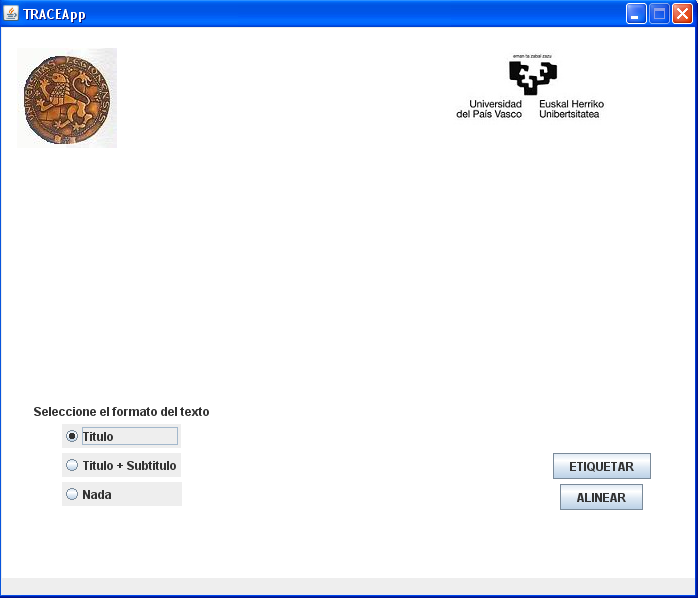
\includegraphics[width=.5\textwidth]{./figures/6-1.png}
\caption{Interface of the tagging/aligning program} \label{fig:3:1}
\end{figure}


The third stage involved aligning the texts: this consisted of three steps: tagging the texts, aligning the texts automatically and fine-tuning the alignment manually. \figref{fig:3:1} shows the interface of \textsc{trace}--aligner, the program we developed to create our subcorpora, which gives access to the main functions: tagging (\textit{etiquetar}) and alignment (\textit{alinear}).\footnote{\textsc{trace}--aligner is written in Java using Eclipse. We work with an Alpha version (\textsc{trace}--aligner 3.0) which we are still testing and developing, but we hope to produce a stable Beta version soon. The “cleaning tool” mentioned above, for instance, is integrated in \textsc{trace}--aligner 3.0.} 

Firstly, each text was automatically annotated in \textsc{xml} by automatically adding paragraph and sentence boundaries, to which a header containing metadata (title, author, translator, code, language, translation mode and genre) was added. Providing the texts with metadata becomes essential to subsequently exploit the corpus, as it allows the definition of subcorpora in the queries, i.e. to only search in assumed direct translations, for example, or only in indirect translations. \figref{fig:3:2} is an example of \textsc{xml} annotation.

\begin{figure}[t]
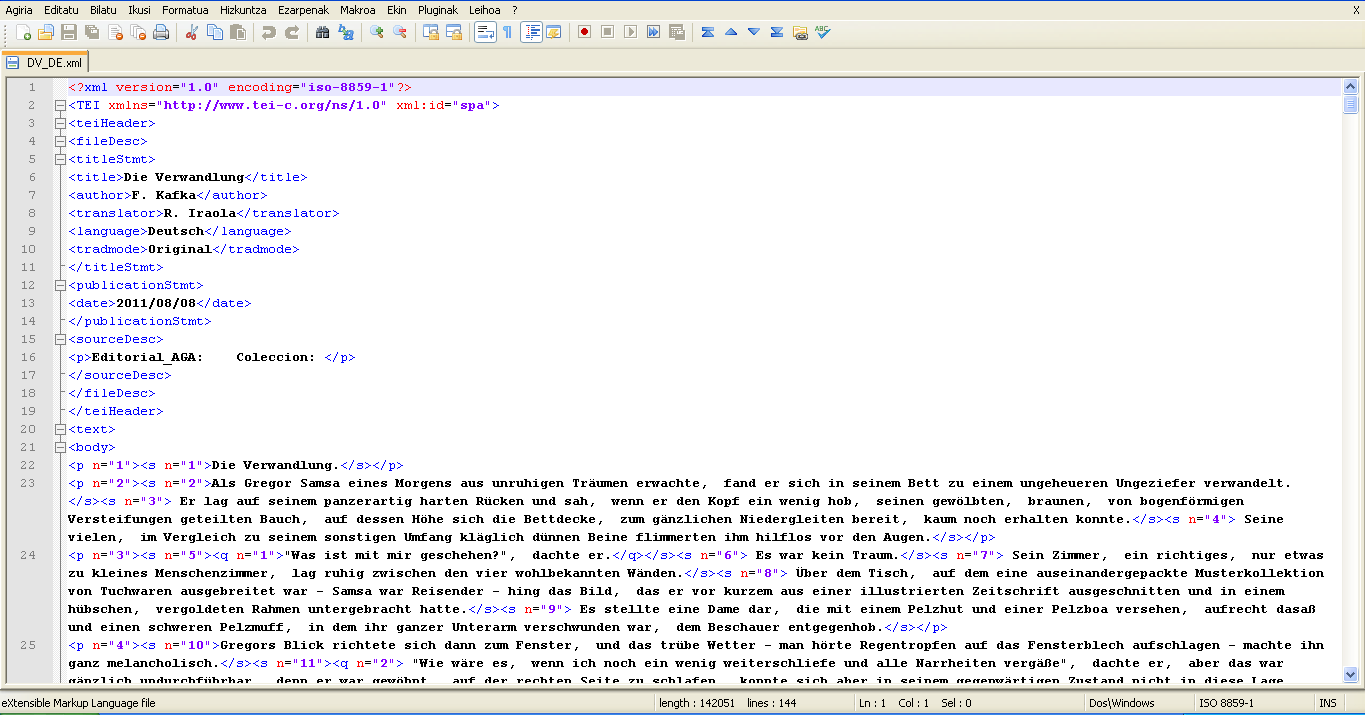
\includegraphics[width=1.0\textwidth]{./figures/6-2.png}
\caption{\textsc{xml} annotation of sample text} \label{fig:3:2}
\end{figure}

Once the texts are annotated, our software tool performs the automatic alignment of the source text and of up to two target texts.\footnote{The latest version of the program, \textsc{trace}--aligner 3.0, can align multiple texts.}  That is, the program will automatically align the tagged \textsc{xml} files at the sentence level. The result can be seen in \figref{fig:3:3}. Given that in any translation process one sentence does not necessarily correspond to another, a third step was necessary: the final fine-tuning using manual alignment.

\begin{figure}[p] 
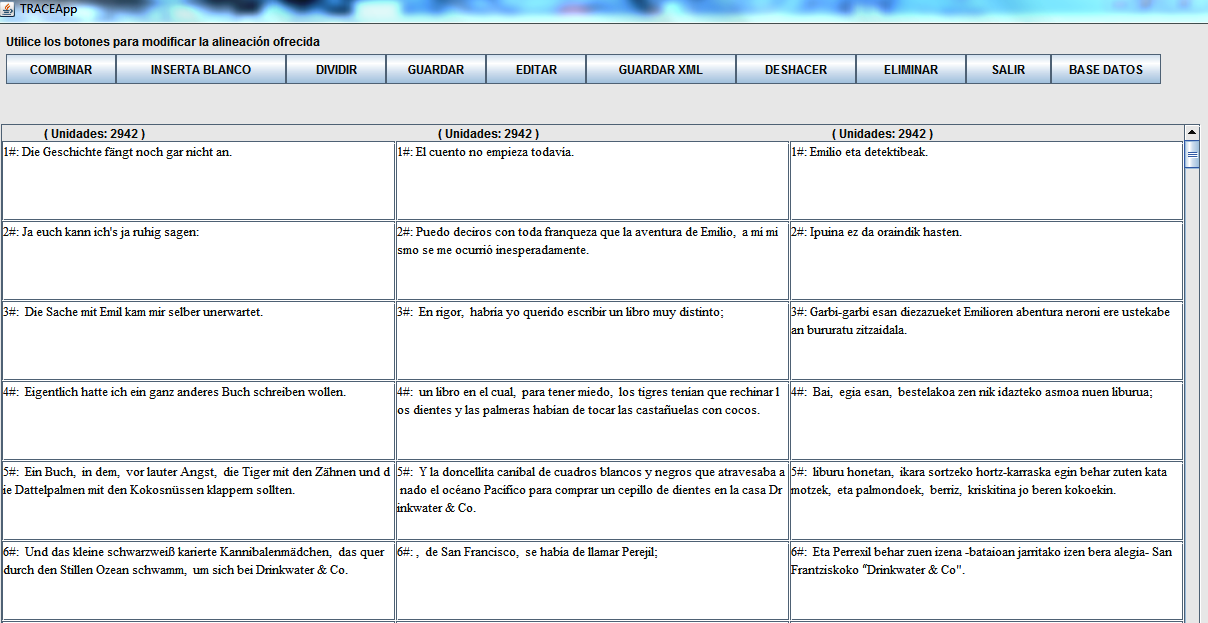
\includegraphics[width=1.0\textwidth]{./figures/6-3.png}
\caption{Sample output of automatic alignment} \label{fig:3:3}
\end{figure}

In order to manually edit the results of automatic alignment, we added different editing options to the program, such as “combine”, “add cell”, “edit” or “split”, to make the tool as versatile and as easy to use as possible. The aim during manual alignment editing was to reflect the structure of the original text. This process is absolutely necessary, as different translations of a source text could vary significantly in terms of syntax and sentential structure, and the results displayed by the search engine depend on the alignment modifications made at this stage in accordance with the source text. The outcome of this process is shown in \figref{fig:3:4}.

\begin{figure}[p]
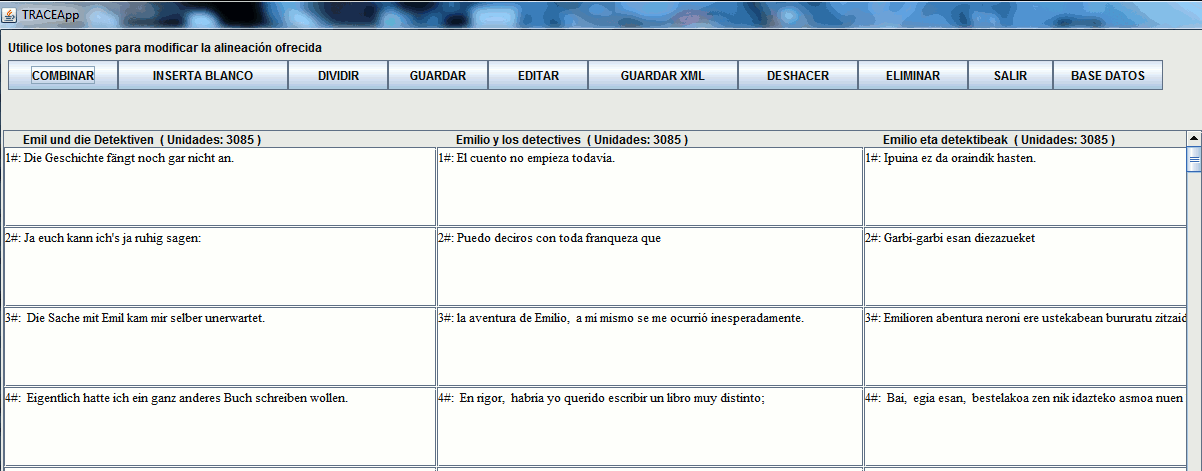
\includegraphics[width=1.0\textwidth]{./figures/6-4.png}
\caption{Sample of output after manual alignment editing} \label{fig:3:4}
\end{figure}

\subsubsection{Making queries in the database} 
The tagging/aligning program allows the user to upload the aligned texts into a MySQL database management system (we used the program Xampp for that purpose). \figref{fig:3:5} shows an image of the database management interface.

\begin{figure} 
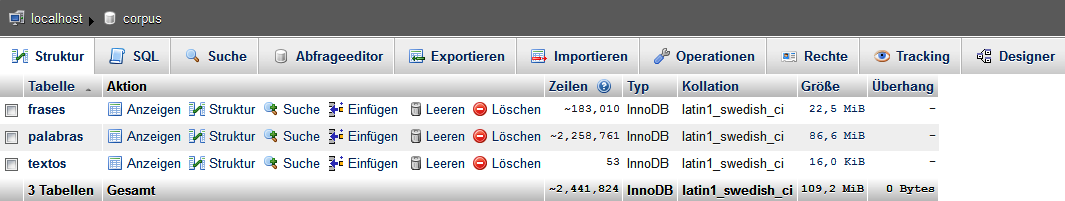
\includegraphics[width=1.0\textwidth]{./figures/6-5.png}
\caption{Image of the MySQL database, where the aligned texts are uploaded} \label{fig:3:5}
\end{figure}

Once the aligned texts are uploaded into the database, it is possible to carry out searches using a specifically developed search engine. The inclusion of metadata associated with each text makes it possible to define specific searches: by defining a given language, searches on the source- or the target-text are possible, or the search can be limited to a specific author or translator. As such, different ad hoc subcorpora can be defined with the search criteria. The search engine interface is shown in \figref{fig:3:6}.


\begin{figure}[b] 
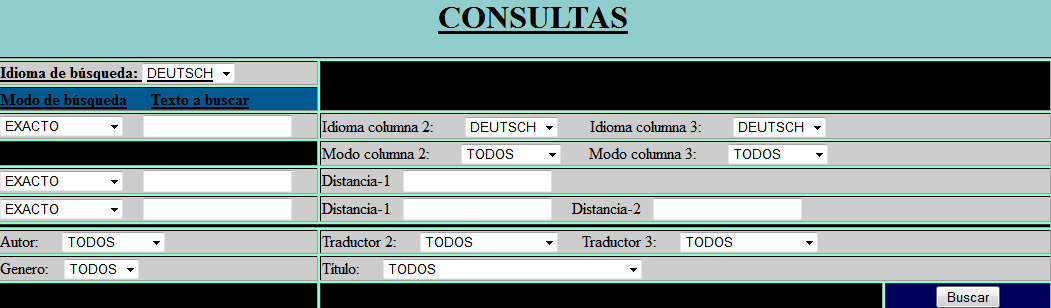
\includegraphics[width=0.9\textwidth]{./figures/6-6.png}
\caption{The search engine linked to the database} \label{fig:3:6}
\end{figure}

\figref{fig:3:7} shows the results of a search as displayed by the search engine. In this example, the search criteria are German sentences containing the words “Nagel” and “Kopf”. The first column contains the code for the aligned texts, the second column the original German text, the third, when applicable, the mediating Spanish texts and the last column the target texts in Basque. Another important feature is that the results are always contextualised: in addition to the sentence containing the words searched for, the preceding and the following sentences are also displayed.

\begin{figure}
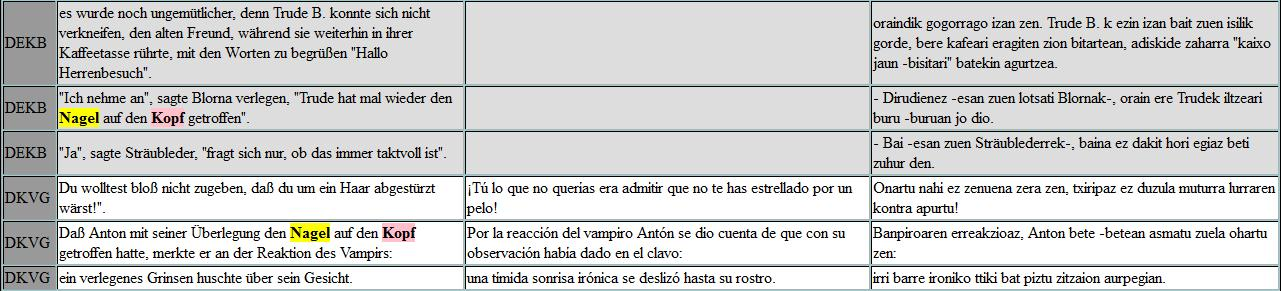
\includegraphics[width=0.9\textwidth]{./figures/6-7.jpg} 
\caption{Example of the results of a search in the corpus} \label{fig:3:7}
\end{figure}

\section{Preliminary results}
As a result of the process described above, we have created a digital, multilingual and parallel corpus, which is relatively small (over 5 million words) and topic-specific. It may not be a large corpus, but given that it was created according to the criteria which suited our research needs (see \sectref{sec:3:2}), it does provide a representative sample of the textual reality we observed. Although the main aim of this article is to describe the process of creating the corpus and the corpus itself,\footnote{We continue to develop \textsc{trace}--Aligner and we hope to incorporate text analysis features in the near future (word count, word lists, word frequencies, automatic extraction of collocations and so on).} this section presents two examples we have extracted from the corpus and which served as data for our research projects to illustrate how the corpus can be exploited.

A first example comes from \citeauthor{Zubillaga2013}'s \citeyear{Zubillaga2013} research on insults in German texts translated into Basque, using the AleuskaHGL subcorpora. In order to search for the most common insults in German, Scheffler's list (2000) was used as a reference. The insults in the list were queried one by one in the search engine and then the results were systematically analysed, paying special attention to cases of standardisation and interference. The following is an example of an indirect translation, that is, the Basque translator never looked at the German, but solely used the Spanish version. The search engine displays the three aligned texts so that we can observe the history of the entire translation process. In this case, the translation was carried out in two separate steps: the work was first translated from German into Spanish, and the Basque translation was conducted three years later, taking the mediating Spanish text as its actual source text. This example, along with various others, was classified as a case of standardisation of an insult.


\begin{table}
     \centering
     \begin{tabularx}{\textwidth}{XXX}
     \lsptoprule
\textsc{ot} 			& \textsc{mt}     & \textsc{tt}  \\ 
\midrule
Mein Kind soll keine \textbf{hochnäsige Gans} werden (Kästner 1931).   & Mi hija no debe convertirse en un \textbf{ganso orgulloso} (Kästner 1987).   & Nire alaba ezin da izan \textbf{antzara harroa} (Kästner 1989). \\ 
{[}My child won't be an arrogant goose. (meaning: \textbf{arrogant}){]} & {[}My daughter won't become an arrogant goose. (meaning: \textbf{an arrogant fool}){]}  & {[}My daughter cannot be an arrogant goose (meaning: \textbf{an arrogant goose}, meaning literally the animal){]}  \\

\lspbottomrule
\end{tabularx}

 \caption{Example of indirect translation}
     \label{3.3}
     % Verweis im Text mittels \REF{tbl:beispieltabelle}
\end{table}


A \textit{hochnäsige Gans} is somebody who is arrogant or stuck-up. The Spanish version uses the equivalent \textit{ganso orgulloso}, which is a literal translation. \textit{Ganso} is an insult in Spanish, but actually has the meaning of somebody foolish, not arrogant, although that is compensated with \textit{orgulloso}, which means arrogant. The Basque version departs from the Spanish version and also gives the literal translation of the Spanish version, i.e. the dictionary equivalent: \textit{antzara harroa}, but \textit{antzara} `goose/Gans' has no insulting connotation in Basque, it just has the literal meaning for that type of animal. The final Basque target text is, therefore, standardised, since we understand that the toning down of the offensive language reveals the standardisation of the same. In this example, the insult is completely lost compared to the mediating Spanish text, and we were able to observe that the meaning of the insult in the Spanish version is somewhat modified compared to the original German text. In summary, the literal translation from German into Spanish modifies the meaning, as \textit{Gans} and \textit{ganso} have different connotations in German and Spanish; and the literal translation of the Spanish version into Basque normalises the special meaning attached to \textit{ganso}, since \textit{antzara} has no association with foolish behaviour as is the case in Spanish, nor does it have any relation to arrogance as in German.

Example 2 arose from the AleuskaPhraseo subcorpora, as \citet{Sanz2014} was conducting her analysis on German Phraseology translated into Basque. The example is from an assumed direct translation; that is, the text had supposedly been translated directly from the German original version, and so we digitised and aligned just the German and the Basque versions.\footnote{Until now, Spanish translations were included in the corpus only when the original texts had been translated through a mediating text. During our research, we realised that it would be very interesting to have the opportunity to consult the Spanish translation in all cases, also when translations were presumably made from the German original, in order to check if there is any relationship between the Spanish and Basque texts. Therefore, the systematic inclusion of the Spanish translations in the corpus is something we intend to do in the future.} This is an example of what we called diglossic interference or interference of the dominant language (Spanish, in this case), as described above.

\begin{table}[t]
     \centering
     \begin{tabularx}{\textwidth}{XX}
     \lsptoprule
German original    & Spanish bridge version  \\ 
\midrule
Kann jedem mal passieren, daß \textbf{ihm die Hand ausrutscht}, wenn er in Rasche ist".	(Döblin 1929).   &  Edonori gertatzen zaiok, amorrazita dagoenean \textbf{eskuak alde egitea}". (Döblin 2000).  \\ 
{[}It can happen to anyone that, when he/she gets angry, his/her hand slips (meaning: someone gives another person a slap in the face){]}  & {[}It can happen to anyone that, when he/she gets angry, his/her hand runs away{]}  \\

\lspbottomrule
\end{tabularx}

 \caption{Example of a diglossic interference}
     \label{3.4}
     % Verweis im Text mittels \REF{tbl:beispieltabelle}
\end{table}     
   
As we can see in the German version, the author uses the German idiom \textit{jmdm rutscht die Hand aus} which -- according to Duden 11, a German monolingual dictionary specialised in German idioms and proverbs -- has the following meaning “jmd. gibt jmdm. eine Ohrfeige”. In other words, the actual meaning of the \textsc{pu} is to give someone a slap in the face, and word for word it can be translated as “someone's hand slips”. In the Basque translation, we do not find a \textsc{pu}. We were not able to find the expression used in the Basque version in any dictionary and when we searched for this word combination (“eskuak alde egin”) in the large corpora mentioned in \sectref{sec:3:1} (\textsc{etc} corpus), we found no occurrences. We believe that the translator has made a literal translation of a Spanish \textsc{pu}, which is “escapársele a alguien la mano”,\footnote{According to María Moliner, a well-known Spanish monolingual dictionary, it means “no poder contenerse de hacer cierta cosa” or not to be able to stop oneself from doing something.} because the Basque version is a "word for word" translation. We cannot explain the process of this translation without taking into account that the translator of this text is a diglossic translator, living in a diglossic community, using indirect tools to translate (i.e. German--Spanish dictionaries first, and Spanish--Basque dictionaries afterwards).\footnote{No German--Basque dictionaries existed at the time of the translation in question.} For these reasons, we consider this to be a case of diglossic interference.

The two cases presented above have shown how we have used the search tool in order to retrieve data from the corpus on the one hand and, on the other, how translation behaviour has been analysed in the framework of our research projects. \tabref{3.3}, in the context of an indirect translation process, shows a case of toning down, which we link with the law of standardisation. \tabref{3.4} represents a case of interference which, however, does not stem from the German source text but rather from the translator diglossic competence. In this and other cases, although the translation was nominally direct from German, the Basque target texts contained interferences from another language, Spanish in our case.

\section{Conclusions}

The aim of this article was to explain and present the steps we undertook to build up our corpora and to report initial results. Thanks to the teamwork with our computer technician, we were able to create a user-friendly program and with its help we can now build up our own digitalised, aligned and searchable multilingual corpora.

On the technical side, we are developing \textsc{trace}--Aligner 3.0. The updated and improved version can now align more than 3 texts and the database production is much simpler. We will next integrate some text analysis features, starting with those present in model tools like AntConc\footnote{\url{http://www.laurenceanthony.net/antconc_index.html}.} and WordSmith Tools. We are also working on the integration of all three existing subcorpora into one general German to Basque parallel corpus consisting of over 5 million words, which will be soon locally available for internal use among researchers of our faculty. The publication of the entire corpus or parts thereof is under consideration, but this move is hindered by copyright issues.

In the matter of use and exploitation, our work is at an early stage; however, we were able to identify both standardisation and interference at work in a context, where the development of a standard form of Basque is an additional factor. Our initial results (for example, regarding different types of interference) now need to be checked with further studies. On the other hand, the process of creating our corpus is a long-term investment which can have many different applications in the future. It can be the departing point for further empirical and systematic research on German to Basque translations and may also play a role in translation didactics, lexicography, contrastive linguistics and other related areas. Our corpus could also serve as a model for similar work with translations from other source languages into Basque and, in the process, could help broaden the picture to the larger field of translations into Basque.


\section*{Acknowledgements}

We would like to thank our computer technician, Iñaki Albisua, who has developed \textsc{trace}--Aligner 2.0 and \textsc{trace}--Aligner 3.0.

\printbibliography[heading=subbibliography,notkeyword=this]

\end{document}

% % copy the lines above and adapt as necessary

%%%%%%%%%%%%%%%%%%%%%%%%%%%%%%%%%%%%%%%%%%%%%%%%%%%%
%%%                                              %%%
%%%             Backmatter                       %%%
%%%                                              %%%
%%%%%%%%%%%%%%%%%%%%%%%%%%%%%%%%%%%%%%%%%%%%%%%%%%%%

% There is normally no need to change the backmatter section
%\input{backmatter.tex} 
\end{document} 

% you can create your book by running
% xelatex main.tex
%
% you can also try a simple 
% make
% on the commandline
